% CVPR 2022 Paper Template
% based on the CVPR template provided by Ming-Ming Cheng (https://github.com/MCG-NKU/CVPR_Template)
% modified and extended by Stefan Roth (stefan.roth@NOSPAMtu-darmstadt.de)

\documentclass[10pt,twocolumn,letterpaper]{article}

%%%%%%%%% PAPER TYPE  - PLEASE UPDATE FOR FINAL VERSION
%\usepackage[review]{cvpr}      % To produce the REVIEW version
\usepackage{cvpr}              % To produce the CAMERA-READY version
%\usepackage[pagenumbers]{cvpr} % To force page numbers, e.g. for an arXiv version

% Include other packages here, before hyperref.
%\usepackage[accsupp]{axessibility}
\usepackage{graphicx}
\usepackage{amsmath}
\usepackage{amssymb}
\usepackage{booktabs}
\usepackage[ruled,vlined]{algorithm2e}
\usepackage{epsfig}
\usepackage{physics}
\usepackage[inline]{enumitem}
\usepackage{comment}
\usepackage{subcaption}
\usepackage{framed}
\usepackage{multirow}
\usepackage{xcolor,soul}
\usepackage{latexsym,url}
\usepackage{stackengine} 

% It is strongly recommended to use hyperref, especially for the review version.
% hyperref with option pagebackref eases the reviewers' job.
% Please disable hyperref *only* if you encounter grave issues, e.g. with the
% file validation for the camera-ready version.
%
% If you comment hyperref and then uncomment it, you should delete
% ReviewTempalte.aux before re-running LaTeX.
% (Or just hit 'q' on the first LaTeX run, let it finish, and you
%  should be clear).
\usepackage[pagebackref,breaklinks,colorlinks]{hyperref}



% Support for easy cross-referencing
\usepackage[capitalize]{cleveref}
\crefname{section}{Sec.}{Secs.}
\Crefname{section}{Section}{Sections}
\Crefname{table}{Table}{Tables}
\crefname{table}{Tab.}{Tabs.}


%%%%%%%%% PAPER ID  - PLEASE UPDATE
\def\cvprPaperID{8360} % *** Enter the CVPR Paper ID here
\def\confName{CVPR}
\def\confYear{2022}

\definecolor{todocolor}{RGB}{200,120,120}
\sethlcolor{todocolor}
\newcommand{\todo}[1]{\textcolor{black}{\hl{#1}}}

\newcommand{\multilineC}[1]{\begin{tabular}[b]{@{}c@{}}#1\end{tabular}}
\newcommand{\multilineCB}[1]{\textbf{\multilineC{#1}}}

% \def\etal{{et.~al}}
% \def\sota{\textsc{sota}\xspace}
% \def\cnn{\textsc{cnn}\xspace}
% \def\usg{\textsc{usg}\xspace}
% \def\gbc{\textsc{gbc}\xspace}
% \def\gb{\textsc{gb}\xspace}
% \def\mri{\textsc{mri}\xspace}
% \def\ct{\textsc{ct}\xspace}
% \def\roi{\textsc{roi}\xspace}
% \def\rois{\textsc{roi}s\xspace}
% \def\gbcnet{\textsc{gbcn}et\xspace}
% \def\mssop{\textsc{MS-SOP}\xspace}


\begin{document}

%%%%%%%%% TITLE - PLEASE UPDATE
%\title{Surpassing the Human Accuracy in Detecting Gallbladder Cancer from USG Images with Deep Neural Networks and Curriculum Learning}
%\title{GBCNet: Surpassing the Human Accuracy in Detecting Gallbladder Cancer from Ultrasound Images with Deep Neural Networks and Curriculum Learning}
%\title{GBCNet: A Three Stage Neural Network Architecture for \\ Detecting Gallbladder Cancer from Ultrasound Images}
\title{Surpassing the Human Accuracy: \\ Detecting Gallbladder Cancer from USG Images with Curriculum Learning}

\author{Soumen Basu\textsuperscript{1}, Mayank Gupta\textsuperscript{1}, Pratyaksha Rana\textsuperscript{2}, Pankaj Gupta\textsuperscript{2}, Chetan Arora\textsuperscript{1} \\
\textsuperscript{1} Indian Institute of Technology, Delhi, India \\ 
\textsuperscript{2} Postgraduate Institute of Medical Education and Research, Chandigarh, India\\
%{\tt\small \href{https://gbc-iitd.github.io/gbcnet.html}{https://gbc-iitd.github.io/gbcnet.html}}
%{\tt\small \{soumen.basu, mayank.gupta, chetan\}@cse.iitd.ac.in}\\
%{\tt\small pratyaksha\_25@yahoo.in, pankajgupta959@gmail.com}
% For a paper whose authors are all at the same institution,
% omit the following lines up until the closing ``}''.
% Additional authors and addresses can be added with ``\and'',
% just like the second author.
% To save space, use either the email address or home page, not both
}

\maketitle

%%%%%%%%% ABSTRACT
%\doublespacing
\onehalfspacing
\pagestyle{plain}
\addcontentsline{toc}{chapter}{Abstract}
\chapter*{Abstract}

Gallbladder Cancer (GBC) is the most common biliary tract cancer and the 5th most common gastrointestinal tract malignancy. India sees about 20\% of annual GBC-related deaths worldwide and faces an incidence rate compared to the global highest. The overall mean survival rate for patients with advanced GBC is only six months, and the 5-year survival rate is less than 5\%. Early diagnosis and curative surgical resection remain the only hope to improve the bleak survival statistics. Ultrasound (USG) is a popular and excellent candidate diagnostic modality for abdominal ailments in low-resource settings due to its low cost, availability, and ionizing radiation-free nature. USG is also the first-line diagnostic modality for gallbladder (GB) diseases. However, diagnosing GBC in USG is difficult, even for experienced radiologists, due to the overlapping visual features of benign and malignant GBs and various confounding medical conditions such as cholecystitis, pancreatitis, and Rokitansky-Aschoff sinuses. Our experiments reveal that human experts could achieve only about 70\% sensitivity (recall) in differentiating GBC from benign diseases (dichotomous classification) from USG. 

\par Inspired by the recent success and the transformational capabilities shown by Machine Learning (ML) models, especially the Deep Neural Networks (DNNs), in a plethora of medical image computing tasks, we investigate leveraging DNNs to detect GBC from USG. However, the low image quality arising from noise and artifacts such as shadows or textures, the operator bias and variation in view due to handheld sensors, and the lack of annotated data make the application of DNNs difficult in USG. 

\par In our pursuit of enhancing diagnostic capabilities, we systematically explore the potential of deep convolutional models, leading to the development of GBCNet. GBCNet is a two-stage DNN that first localizes the GB or the region-of-interest (ROI), and then employs a specialized classifier based on multi-scale, second-order pooling (MS-SoP) for robust GBC detection. We further develop a Gaussian smoothing-based training curriculum inspired by human visual acuity to mitigate the effect of spurious textures. GBCNet tackles issues such as noise, artifacts, and viewpoint variation in USG imaging, improving the GBC detection sensitivity by 7 points compared to SOTA DNN models and 20 points compared to expert radiologists. 

\par The reliance on bounding box annotations for training GBCNet's localization component presents a significant bottleneck, given the high cost and complexity of obtaining such annotations. To overcome this challenge, we utilize limited supervised data by introducing -- (1) an unsupervised contrastive framework for learning GBC representations from unlabelled videos, and (2) a weakly supervised object detection technique to use only image labels instead of bounding box annotation requirements, thus designing more practical models for real-world deployment. 

\par We address the crucial aspect of interpretability in GBC detection by introducing RadFormer, a deep neural network architecture capable of generating interpretable explanations for its decisions. RadFormer not only improves detection sensitivity over GBCNet but also aids in understanding the underlying visual features relevant to GBC diagnosis, bridging the gap between AI-based detection and clinical interpretability. 

\par Finally, we advocate for a paradigm shift towards video-based GBC detection, leveraging the rich spatiotemporal information available in full USG videos. Video-based detection is also clinically more relevant as single frames may not contain conclusive evidence for disease detection. We introduce an innovative masked auto-encoder design called FocusMAE, to learn self-supervised representations for GBC from USG videos. We demonstrate significant improvements in GBC detection using FocusMAE, achieving a 100\% sensitivity and thus showcasing the potential of video-based approaches in streamlining the detection process and reducing operator-specific variations.

\par In summary, we designed and developed accurate, data-efficient, interpretable, and clinically relevant DNN models which could overcome the challenges such as noise, artifacts, viewpoint variability, data scarcity, and real-time applicability in detecting GBC from USG, thereby opening future avenues for transformational research.

% Gallbladder Cancer (GBC) is the most common biliary tract cancer and the 5th most common gastrointestinal tract malignancy. India sees about 20\% of annual GBC-related deaths worldwide and faces an incidence rate compared to the global highest. The overall mean survival rate for patients with advanced GBC is only six months. Early diagnosis and curative resection remain the only hope to improve the outcomes. Ultrasound Sonography (USG) is a popular and excellent candidate diagnostic modality for abdominal ailments in low-resource countries. However, the clinical characterization of GBC in USG is difficult, even for experienced radiologists. The low image quality due to noise and artifacts, and the variation in view due to handheld sensors, make automated detection difficult. In this work, we investigate leveraging Deep Neural Networks (DNNs) to detect GBC from USG and tackle the challenges posed by USG. 

% We first address inherent issues in ultrasound images — noise, shadows, and spurious textures- and develop a robust model (GBCNet) to improve the accuracy of predictions significantly. Our focus then extends to improving interpretability in model decisions, introducing RadFormer to provide insights behind predictions, and enhancing its practicality in clinical settings. Additionally, we explore a pivotal challenge in medical computer vision — learning from limited supervised data and developing a self-supervised contrastive pretraining framework. We also leverage the USG video data to build a robust model for GBC detection in videos, eliminating the manual frame selection by radiologists and streamlining the entire detection process.

%%%%%%%%% BODY TEXT
\begin{figure}[t]
    \centering
    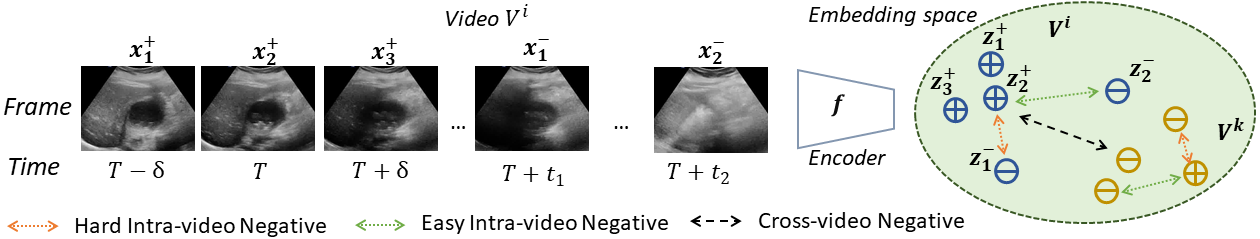
\includegraphics[width=\linewidth]{figs/teaser.png}
    \caption{(a), (b), and (c) Normal, benign, and malignant \gb sample in \usg images, respectively. While normal or benign \gb have regular anatomy, clear boundary is absent in malignant \gb. (d) A malignant (biopsy-proven) \gb sample. (e) Shadows having visual traits of a \gb leads to localization error in ResNet50. (f) \gbcnet tackles shadow artifacts well. (g) Another sample of malignant \gb. (h) The radiologist incorrectly diagnosed the \gb as benign based on the stone and wall thickening. (i) \gbcnet helps the radiologist to identify the salient region with liver infiltration by the \gb, a critical feature of \gbc, and correct the prediction.}
    \label{fig:teaser}
\end{figure}


\section{Introduction}
%
According to GLOBOCAN 2018 \cite{bray2018global}, worldwide about 165,000 people die of \gbc annually. For most patients, \gbc is detected at an advanced stage, with a mean survival rate for patients with advanced \gbc of six months and a 5-year survival rate of 5\% \cite{randi2006gallbladder, gupta2021locally}. Detecting \gbc at an early stage could ameliorate the bleak survival rate. 

Lately, machine learning models based on convolutional neural network (\cnn) architectures have made transformational progress in radiology, and medical diagnosis for diseases such as breast cancer, lung cancer, pancreatic cancer, and melanoma \cite{ardila2019end, bejnordi2017diagnostic, chu2019application, codella2017deep, han2017breast}. However, their usage is conspicuously absent for the \gbc detection. Although there has been prior work involving segmentation and detection of the \gb abnormalities such as stones and polyps \cite{gbPolyp, gbPolyp2, gbAutomatic}, detection of \gbc is missing from the list. A search on Google Scholar with keywords ``artificial intelligence'' and ``gallbladder cancer'' returned 204 articles between 2015-2021. In these, we did not find any published article on deep learning-based \gbc detection from \usg images.

%\par According to GLOBOCAN 2018, GBC causes 165,087 deaths and 219,420 incidences every year worldwide \cite{armitage2014abeloff, bray2018global}. 
%%GBC is one of the leading causes of cancer-related deaths among Indian women \cite{randi2006gallbladder, bray2018global}. 
%The disease is prevalent in China, India, and Latin America. Canada, Australia, USA, and Europe also face a high incidence of GBC. 
%%\figref{fig:sec1-1} shows the detailed distribution of the incidence rate around the world.  
%GBC is detected at an advanced and metastasized stage for most patients, impeding curative resection and resulting in a dismal prognosis \cite{randi2006gallbladder, gupta2021locally}. 
%The overall mean survival rate for patients with advanced GBC is six months, with a 5-year survival rate of 5\%. 
%%In the USA, only about 1 in every 5 cases of GBC are identified in an early stage \cite{howlader2017seer}.
 
Early diagnosis and resection are critical for improving the survival rate of \gbc. Due to the non-ionizing radiation, low cost, portability, and accessibility, \usg is a popular diagnostic imaging modality. Although identifying anomalies such as stones or \gb wall thickening at routine \usg is easy, accurate characterization of the wall thickening is challenging \cite{gupta2020imaging, gb-rads-paper}. Often, \usg is the sole diagnostic imaging performed for patients with suspected \gb ailments. If malignancy is not suspected, no further testing is usually performed, and \gbc could silently advance. Therefore, it is imperative to develop and understand the characterization of \gb malignancy from \usg images.

There are significant challenges in using \cnn models for \usg image analysis. Unlike \mri or \ct, \usg images suffer from low imaging quality due to noise and other sensor artifacts. The views are also not aligned due to the handheld nature of the sensor. We observe that modern \cnn classifiers fail to localize the salient \gb region due to the presence of shadows which often have similar visual traits of a \gb in \usg images (\cref{fig:teaser}). Training object detectors for \gbc detection gets biased towards learning from spurious textures due to noise and adjacent organ tissues rather than the shape or boundary of \gb wall, which results in poor accuracy. Further, unlike normal and benign \gb regions, which have regular anatomy, malignant cases are much harder to detect due to the absence of a clear \gb boundary or shape and the presence of a mass.

\mypara{Contributions} 
%
The key contributions of this work are:
%\vspace{-0.5em}
\begin{enumerate}%[label=\textbf{(\arabic*)}]
%\itemsep-0.5em
	\item We focus on circumventing the challenges for automated detection of \gbc from \usg images and propose a deep neural network, GBCNet, for detecting \gbc from \usg images. GBCNet extracts candidate regions of interest (\rois) from the \usg to mitigate the effects of shadows and then uses a new  multi-scale, second-order pooling-based (MS-SoP) classifier on the \rois to classify gallbladder malignancy.
    %The first two stages of GBCNet are inspired by two-stage object detectors but focus only on detecting the \gb (and not cancer) and selecting a focused region of interest (\roi) to mitigate the effects of shadows. The third stage uses a new multi-scale, second-order pooling (MS-SoP) architecture to classify gallbladder malignancy.
	MS-SoP encodes rich feature representations for malignancy detection. 
	%
	\item Even though GBCNet shows improvement in \gb malignancy detection over multiple \sota models, the spurious texture present in an \roi bias the classification unit towards generating false positives. To alleviate the issue, we propose a training curriculum inspired by human visual acuity \cite{kwon2016compensation, vogelsang2018VisualAcuity}. Visual acuity refers to the sharpness of visual stimuli. %Studies suggest that an initial period of low visual acuity followed by high visual acuity helps the visual cortex in humans to formulate a better receptive field and emphasizes features such as shape or structure while identifying objects. 
	The proposed curriculum mitigates texture bias and helps GBCNet focus on shape features important for accurate \gbc detection from \usg images.% We validate the same in the context of \gbc detection from \usg images. %only, where we show in our experiment that our model after training with the proposed curriculum better focuses on GB boundaries.
	%
	\item A lack of publicly available \usg image datasets related to \gb malignancy adds to the difficulty of utilizing \cnn models for detecting \gbc. We have collected, annotated, and curated a \usg image dataset of 1255 abdominal \usg images collected from 218 patients. We refer this dataset as the Gallbladder Cancer Ultrasound (GBCU) dataset.
	%The dataset is available to the community.
	%post-acceptance of the paper after signing the necessary privacy agreement with our hospital. 	
\end{enumerate}

%
\begin{figure*}[t]
	\centering
	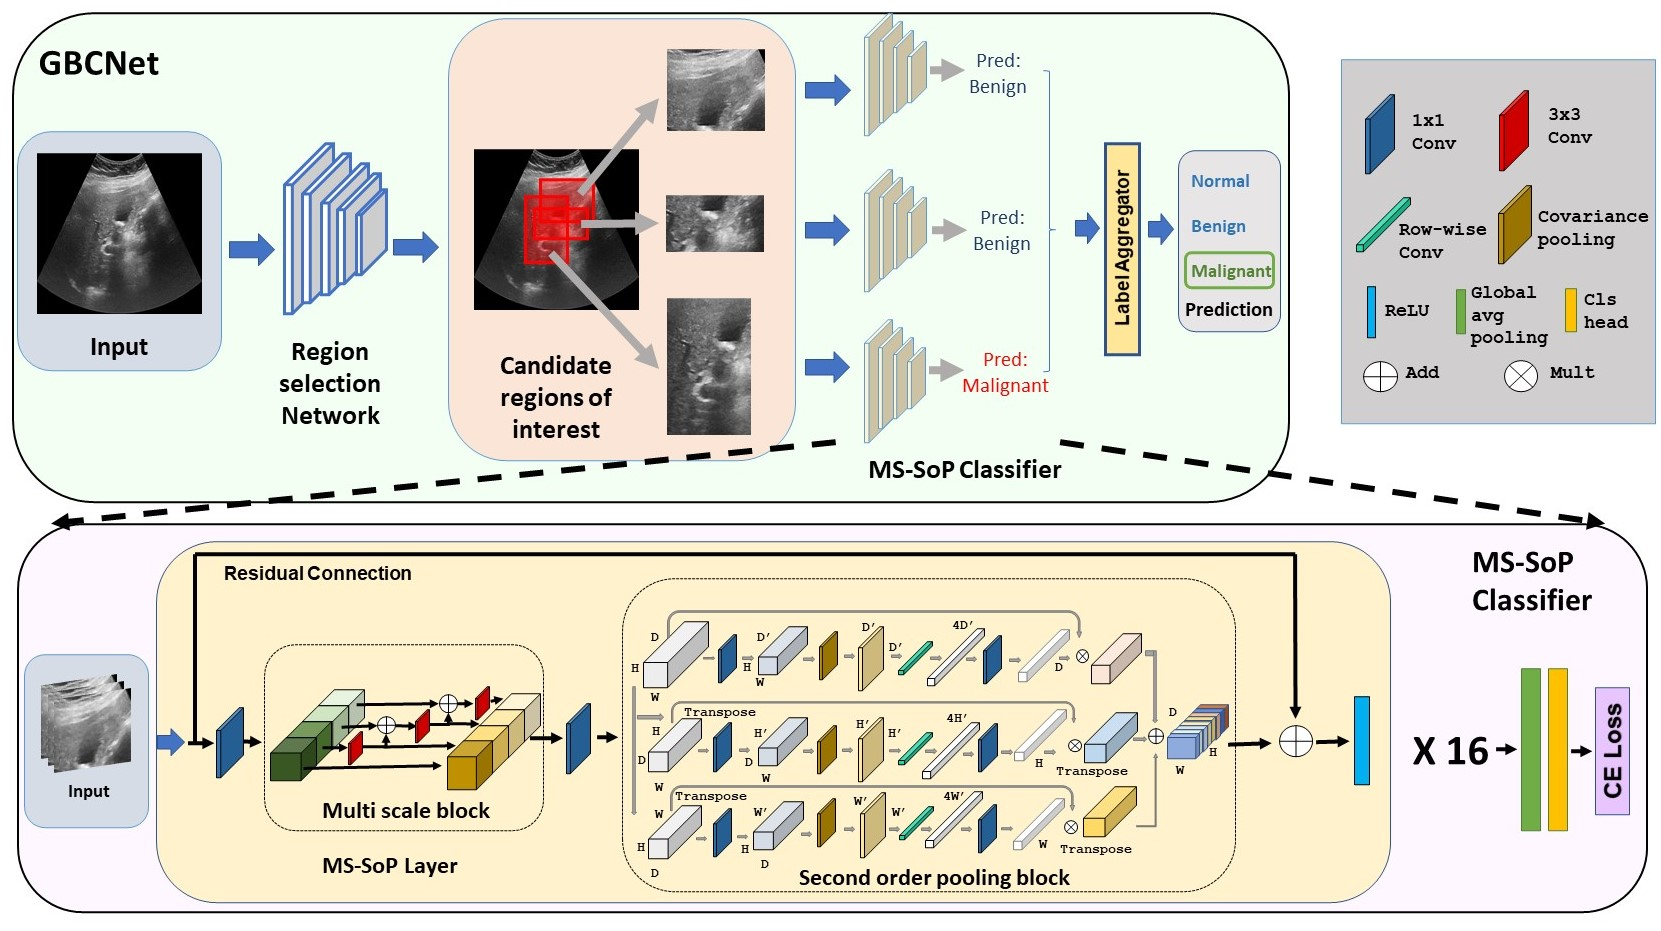
\includegraphics[width=\textwidth]{./figs/arch-compact.jpg}
	\caption{Overview of the \gbcnet architecture. The region selection network localizes the candidate regions of interest and the multi-scale, second-order pooling-based (MS-SoP) classifier at the next stage predicts malignancy for each region. The predictions for each region is aggregated to get the final prediction on the whole image.}
	\label{fig-arch-overview}
\end{figure*}
%

\section{Related Work}

\myfirstpara{Deep Learning for GB Abnormalities}
%
\usg imaging is an effective modality for diagnosing \gbc and related \gb afflictions \cite{yuan2018gbcManual}. 
%Recently, deep learning has been used as a diagnostic tool in medical imaging to great effect \cite{litjens2017dlmedical}. 
%Multiple studies have shown the application of these techniques on GB-related ailments, such as the detection of GB stones, biliary artesia, cholecystitis, and polyps. 
Lien \etal \cite{gbAutomatic} use a parameter-adaptive pulse-coupled neural network for \gb stone segmentation in \usg images. Pang \etal \cite{gbYolo} identify \gb and gallstones using a YOLOv3 model from \ct images. %Chen \etal \cite{gbPolyp} suggest an approach that segments the GB region followed by an AdaBoost classifier for diagnosing polyps. 
Jeong \etal \cite{gbPolyp2} uses an InceptionV3 model to classify neoplastic polyps from cropped samples of \gb \usg images. \gbc is a serious problem affecting a significant number of people. Despite the presence of numerous studies on using deep learning on other \gb-related afflictions, there is an absence of any work that applies deep learning to \gbc detection.

\mypara{Deep Learning for USG}
%
\cnn models have been widely applied in a plethora of \usg-based imaging tasks.
Mishra \etal proposed a fully convolutional neural network with deep attentional supervision on USG images for segmentation of blood vessel, liver lumen, and lesion \cite{mishra2018USSegmentation}. Deep learning-based segmentation models such as U-Net or Link-Net have been used to measure head circumference in fetal USG images \cite{budd2019FetalHC, sobhaninia2019FetalHC}. %VGG16-based architectures have been used for detecting the fetal scan plane \cite{baumgartner2017PlaneDetection}. 
Azizi \etal proposed a Deep Belief Network for detecting prostate cancer from USG images \cite{azizi2015ultrasound}. Li \etal modified Faster-RCNN for improving the detection of papillary thyroid cancer from USG \cite{li2018improved}. Deep learning has also been used in ovarian cancer \cite{zhang2019improved}, metastatic lymph node \cite{lee2018deep}, and breast cancer detection \cite{almajalid2018development, becker2018classification, cao2019BreastLesion, yap2018breast}. Zhu \etal recently proposed an attention-guided second-order sub-region pooling network for exploiting higher-order correlation to extract complex features from USG images \cite{zhu2020second}. A study by Ning \etal implemented a multi-scale higher-order pooling-based solution for breast lesion classification on USG images \cite{ning2020multi} .
%\cnn models have been widely applied in \usg imaging tasks, such as ovarian cancer detection \cite{zhang2019improved}, breast cancer region, mass and boundary detection \cite{bian2017boundary, cao2019BreastLesion, yap2018breast, ning2020multi, zhu2020second}, measuring head circumference in fetal \usg images \cite{sobhaninia2019FetalHC, budd2019FetalHC}. %, and other medical imaging and diagnostic applications. 

%\cite{mishra2018USSegmentation} proposed a fully convolutional neural network with deep attentional supervision on USG images for segmentation of blood vessel, liver lumen, and lesion. Deep learning-based segmentation models such as U-Net or Link-Net have been used to measure head circumference in fetal USG images \cite{sobhaninia2019FetalHC, budd2019FetalHC}. VGG16-based architectures have been used for detecting the fetal scan plane \cite{baumgartner2017PlaneDetection}. \cite{azizi2015ultrasound} proposed a Deep Belief Network for detecting prostate cancer from USG images. \cite{li2018improved} suggested modifications to Faster-RCNN for improving the detection of papillary thyroid cancer from USG. Deep learning has been used in ovarian cancer \cite{zhang2019improved}, metastatic lymph node \cite{lee2018deep}, and breast cancer detection \cite{cao2019BreastLesion, yap2018breast, almajalid2018development, becker2018classification}. \cite{zhu2020second} suggested an attention-guided second-order sub-region pooling network for exploiting higher-order correlation to extract complex features from USG images. A study by \cite{ning2020multi} proposes a multi-scale higher-order pooling-based solution for breast lesion classification on USG images. \cite{wang2020auto} used reinforcement learning to auto-assign weights to multimodal USG framework. 

\mypara{Curriculum Learning}
%
Curriculum learning has been applied to different medical imaging tasks. While Jesson \etal \cite{jesson2017cased} used a patch-based curriculum for lung nodule detection, Tang \etal \cite{tang2018attention} used disease severity level to identify thoracic diseases from chest radiographs. Oksuz \etal \cite{oksuz2019automatic} proposed image corruption-based curriculum to detect motion artifacts in cardiac \mri. 

\mypara{Texture Bias in Neural Networks}
%
Presence of mass and a thickened \gb wall are prominent indicators of \gb abnormality. However, typical \cnn-based architectures are biased towards textures rather than shape \cite{geirhos2018Texture}. This may lead GBCNet to focus on soft tissue textures such as liver rather than noticing cues based on the shape and wall of the \gb. 
%Therefore, a strategy is needed to reduce this texture bias of the network. 
Multiple works have attempted to reduce texture bias and improve the spatial understanding of a model. Geirhos \etal \cite{geirhos2018Texture} suggest style transfer to replace the original texture of images while Brendel \etal \cite{brendel2019BagOfFeatures} propose a method similar to a Bag of Features model to force spatial learning. 

\mypara{Visual Acuity in Learning Models}
%
Vogelsang \etal \cite{vogelsang2018VisualAcuity} suggest that a period of low visual acuity (blurred vision) followed by high visual acuity induces better spatial processing and also increases the receptive field in human vision. 
%Some recent works seem to follow the broad strategy and overcome the texture bias problem using blurring or similar other operations. 
Different from our visual acuity-inspired strategy of working with input space, Sinha \etal \cite{sinha2020curriculumBySmoothing} propose applying a Gaussian kernel on the output feature map of every layer of a network. The use of blurring before pooling seems to mitigate aliasing effects due to sub-sampling in the pooling layer rather than the use of visual acuity. Azad \etal \cite{azad2020textureDoG} have integrated a Difference of Gaussian (DoG) operation into their model. Similar to \cite{sinha2020curriculumBySmoothing}, they end up attenuating the high frequency in the feature maps corresponding to every layer rather than the input image, for which there is no obvious biological connection known. On the other hand, our proposed visual acuity-based curriculum works in the input space and has a solid neural basis \cite{vogelsang2018VisualAcuity}.

\section{Proposed Method}
\begin{figure*}[t]
    \centering
    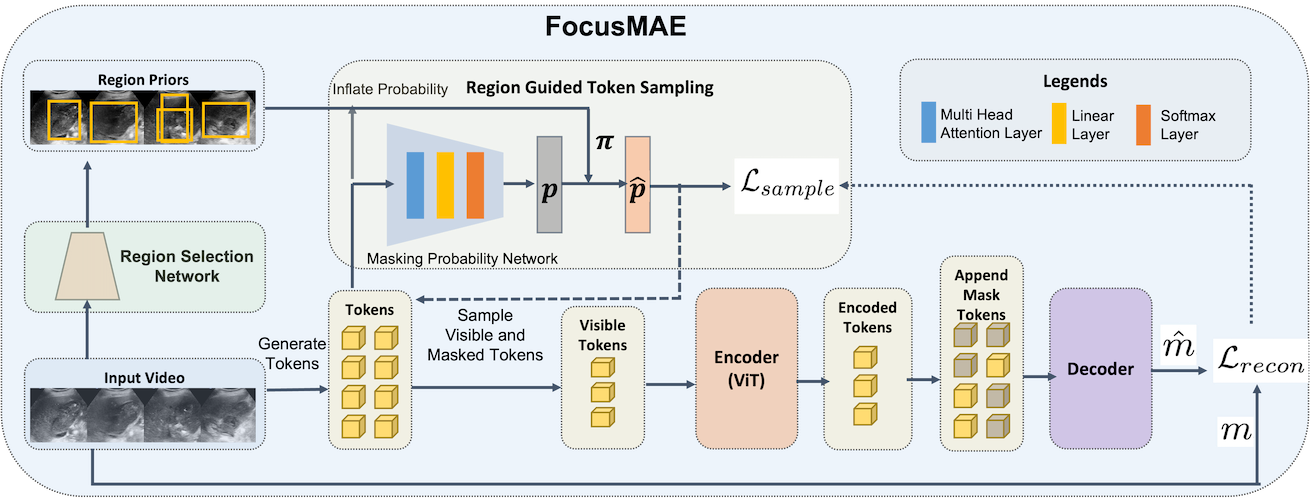
\includegraphics[width=\textwidth]{figs/focusmae/arch.png}
    \caption[Overview of the FocusMAE pipeline]{Overview of the FocusMAE pipeline. Our design proposes guiding the masking tokens with the localization of the candidate focus regions containing high-information. The systematic biasing with focused high-information region priors helps to build a more meaningful reconstruction task for disease representation learning. }
    \label{focusmae_fig:arch}
\end{figure*}

\subsection{Object Priors in MAE}
%
Visual data often demonstrate sparser semantically meaningful information distribution dominated by the foreground objects. Current MAE techniques predominantly use random masking, which may result in sub-optimal performance as the information may not be uniformly distributed. For the USG videos, GBC often occupies a very small portion of the frames. Random masking mostly biases the networks to learn representations of redundant backgrounds containing other organs or abdominal cavities. To alleviate the issue, %we advocate exploiting the object location priors with high information density to enhance the representation learning in MAE. 
we advocate leveraging the object localization priors characterized by high information density to enhance the representation learning in MAE.
We show in \cref{focusmae_fig:teaser_b} the preliminary evidence of potential advantages of boosting the masking token probability with object localization priors. We selected a random validation split containing about 20\% of our GB USG Video dataset. We used the malignant ROI boxes provided in the dataset to specify object locations. We manually increased the masking probability of patches within the bounding box region for the data samples, and used them for self-supervised pretraining. We varied the probability boosting values, denoted by $\pi$, representing the increased probability for patches within the bounding box region as compared to the patches from the background. Our experiment reveals that elevating the probability of masking for patches from the bounding box region, as opposed to random masking, leads to a noticeable enhancement in results. %However, highly inflating the masking probability for patches from the bounding box region may compromise the integrity of the pretext task and result in performance degradation. 
However, excessively inflating the masking probability for patches from the bounding box region may compromise the integrity of the pretext task and consequently lead to performance degradation.
These findings underscore the importance of recognizing that distinct image patches contribute differently to the learning of visual representations. Furthermore, the emphasis on reconstructing foreground objects with a balanced approach is crucial for optimal performance.

\subsection{\focusmae Architecture}
%
\label{sec:method_subsample}
\mypara{Video Sub-sampling}
% 
Video data contains temporal redundancy as the consecutive frames see a very high overlap in content. We sub-sample the videos to reduce the temporal redundancy. Assuming a video containing $F$ frames, we first sub-sample $\frac{F}{4}$ frames with a stride of $4$. Although the viewpoint in USG frames can change very quickly, in our observation of the data, the changes within the frames at a distance equivalent to a stride of 4 from each other are insignificant. Each frame has a size of $3\times H\times W$, $H$, and $W$ stands for the height and width of the frame having three channels (RGB). We further divide these sub-sampled frames for a video into clips -- each clip containing 16 frames. We then randomly sample four clips to use during the pretraining phase. Before passing to the pretraining pipeline, the frames are resized to $224\times 224$.

\mypara{Token Generation}
% 
We first divide a video $V$ of size $T\times 3\times H\times W$ into non-overlapping cubic tokens of size $2\times 3 \times 16 \times 16$. $T$ is the number of frames (temporal dimension), $H$ and $W$ are the height and width of the frames. Each frame has RGB channels. We use a 3D convolution of kernel size = $(2, 3, 16, 16)$,  stride $(2, 16, 16)$, and $d$ output channels. Using this 3d convolution layer, we generate a total of $N=\frac{T}{2}\times\frac{H}{16}\times\frac{W}{16}$ tokens, each of dimension $d$ ($d=384$ in our design) for every video. 
%Next, we add the positional information to the tokens using the fixed 3D periodic positional encoding scheme introduced in \cite{vaswani2017attention}.
Subsequently, we incorporate positional information into the tokens utilizing the fixed 3D periodic positional encoding as introduced in \cite{vaswani2017attention}.

\mypara{Generating Object Localization Priors}
%
We employ deep object detection networks as the region proposal network (RPN) to detect the potential gallbladder region within a frame. The predicted bounding boxes are used as potential candidate regions containing the objects (malignancy). We used the public GBCU \cite{basu2022surpassing} dataset for training the object detectors. The GBCU dataset provides USG images with regions-of-interest marked with bounding boxes. The training focuses on two classes: background and the GB region. We lower the confidence threshold of the predicted boxes to generate multiple candidate regions. These regions are used as priors in a masking token sampler to boost the masking probability of the tokens. If a token's spatial central point falls within the region prior, then its masking probability is inflated. To define a candidate region for an entire clip, we take the union of the candidate regions for each frame within the clip.

\mypara{Masked Token Sampling with Region Priors}
%
To generate the masking probabilities for the tokens, we follow \cite{adamae} and use an auxiliary network consisting of Multi-Head Attention (MHA) with a Linear and a Softmax ($\sigma$) layer following it. Given the embedded tokens $x \in \mathbb{R}^{N \times d}$, the probability scores $p \in \mathbb{R}^N$ over all tokens is generated as follows:
\begin{align}
z = \text{MHA}(x); \quad z \in \mathbb{R}^{N \times d} \\
p = \sigma(\text{Linear}(z)); \quad p \in \mathbb{R}^N
\end{align}
Region priors then boost the probability score as follows:
\begin{align}
\hat{p}_i = p_i + \pi_i 
\end{align}
If the $i$-th token spatially lies within the candidate regions, then we inflate the masking probability of the token by $\pi_i \in(0,\delta)$, where $\delta$ is a small fraction less than $0.25$. 
Subsequently, we choose a set of visible token indices $\mathcal{V} \in {1,\ldots,N}$ without replacement, with a probability of $(1-\hat{p}_i)$ for the $i$-th token. The set of masked token indices, denoted by $\mathcal{M}$, is derived from the complement set of $\mathcal{V}$ within the range ${1,\ldots,N}$, and is given by $\mathcal{M} = \{1,\ldots,N\} \setminus \mathcal{V}$. The number of sampled visible tokens, denoted as $N_v$, is calculated as $N(1 - \rho)$, where $\rho \in (0, 1)$ is a predefined masking ratio. 
%We then select without replacement a set of visible token indices $\mathcal{V} \in \{1,\ldots,N\}$ with the probability $(1-\hat{p}_i)$ for the $i$-th token. The set of masked token indices is given by $\mathcal{M} = \{1,\ldots,N\} \setminus \mathcal{V}$. The number of sampled visible tokens $N_v$ is computed based on a pre-defined masking ratio $\rho \in (0, 1)$ and equals $(1 - \rho)N$.

\mypara{Encoder}
%
For computational efficiency, only the visible tokens are passed to the encoder. The number of visible tokens is $N_v = (1-\rho)N$. We employed a vanilla ViT architecture with space-time attention \cite{timesformer}. The ViT encoder has a depth of 12 layers with 6 heads in each layer. The embedding dimension is 384. 

\mypara{Decoder}
%
The encoded visible tokens are appended with the masked token before passing to the decoder. We keep the decoder depth to 10 after grid searching for optimal depth. The masked tokens are learnable. Usually, the decoder in an MAE architecture is a shallow and narrow ViT. However, our experiments indicate that increasing the decoder depth can help in performance gain. The decoder takes the encoded tokens with the learnable masked tokens and reconstructs the original video cube of size $\frac{T}{2}\times\frac{H}{16}\times\frac{W}{16}$.

\subsection{Training}
%
We use two different loss functions in the \focusmae pre-training phase. The masking reconstruction loss is the primary objective for the MAE-based pre-training framework. On the other hand, we employ a token sampling loss to generate the token sampling probability. At the fine-tuning stage, a cross-entropy loss is used (refer to \cref{sec:focusmae_impl}).

\mypara{Masking Reconstruction Loss} 
%
We have employed the \emph{Mean Squared Error} loss (MSE), measuring the disparity between the predicted and ground-truth RGB values of the masked tokens, as the objective function for pretraining the MAE. The loss function is given as:
\begin{align}
   \mathcal{L}_{recon} = \frac{1}{|\mathcal{M}|}\sum_{i \in \mathcal{M}}||\hat{m}_i - m_i||_2 
\end{align}
Here $\hat{m}$ and $m$ denote the predicted RGB values and the normalized ground-truth RGB values of the token, respectively. $|\mathcal{M}| = \rho N$ refers to the number of masked tokens. %The normalization is done at the patch level, with the mean and variance of the patch.

\mypara{Token Sampling Loss}
%
We use a token sampling loss, $\mathcal{L}_{sample}$, to train the sampling network that generates the sampling probability. We adapt the sampling loss proposed by AdaMAE \cite{adamae} and use maximization of the average reconstruction error to define the loss. The formulation of such a formulation is motivated by the expected reward maximization of the REINFORCE algorithm. %Here, the visible token sampling process is the \emph{action}, the MAE is the \emph{environment}, and the masked token reconstruction error is the \emph{return}. The reconstruction error is high in the high information regions as compared to the low information background regions. Thus, maximizing the expected reconstruction error would result in the network predicting a higher probability score for a high information region. 
In this context, the sampling process of visible tokens serves as the \emph{action}, the MAE acts as the \emph{environment}, and the error in masked token reconstruction represents the \emph{return}. Notably, the reconstruction error tends to be more pronounced in high-information regions compared to low-information background areas. Consequently, maximization of the expected reconstruction error would prompt the network to assign a higher probability score to a high-information region. The loss formulation is as follows:
\begin{align}
    \mathcal{L}_{sample} = - \sum_{i\in \mathcal{M}} \big(\log{\hat{p}_i} \cdot ||\hat{m}_i - m_i||_2 \big)
\end{align}
One key difference with the loss in AdaMAE is that the token probability in our formulation is augmented by the region priors, while AdaMAE uses a token probability for a distribution over the entire image. Thus, we obtain a more refined version of the adaptive token sampling. The log probability tackles the underflow and floating point errors. The gradient flow in the sampling network is kept independent from the ViT encoder and decoder of the main MAE. 
\myfirstpara{Multi-Scale Block}
%
Abdominal organs can appear in significantly different sizes in a \usg image based on the insonation angle or the pressure on the transducer. Perceiving information across multiple scales is thus necessary for accurate \gbc detection. Recently, Gao \etal \cite{res2net} have replaced the standard convolution block in the bottleneck layer with group convolution to add a multi-scale capability to the ResNet architecture. Inspired by \cite{res2net}, we used a hierarchy of convolution kernels on slices of feature volumes in the intermediate layers to capture multi-scale information through a combination of different receptive fields. We split a feature map volume, $\mathcal{X} \!\in\!\mathbb{R}^{H\!\times\! W \!\times\! D}$ ($H, W ~\text{and}~D$ are the height, width, and the number of channels, respectively), depth-wise into 4 slices, $\mathcal{X}_1,\mathcal{X}_2,\mathcal{X}_3$, and $\mathcal{X}_4$, where $\mathcal{X}_i \!\in\! \mathbb{R}^{H\!\times\! W\!\times\! D/4}$. Each $\mathcal{X}_i$ will generate an output split $\mathcal{Y}_i$. The final output, $\mathcal{Y}$, is obtained by concatenating the splits. Suppose $\mathcal{C}_j$ are $3\!\times\!3$ convolution kernels and $\oast$ denotes the convolution. We get each $\mathcal{Y}_i$ as follows:
\linebreak
\begin{minipage}{.4\linewidth}
\vspace{-1em}
\begin{align}
    \mathcal{Y}_1 &= \mathcal{X}_1 \\
    \mathcal{Y}_2 &= \mathcal{C}_1 \oast \mathcal{X}_2
\end{align}
\end{minipage}
\begin{minipage}{.6\linewidth}
\vspace{-1em}
\begin{align}
    \mathcal{Y}_3 &= \mathcal{C}_2 \oast (\mathcal{X}_3 \!+\! \mathcal{Y}_2) \\
    \mathcal{Y}_4 &= \mathcal{C}_3 \oast (\mathcal{X}_4 \!+\! \mathcal{Y}_3)
\end{align}
\end{minipage}

\mypara{Second-order Pooling Block}
%
Traditional average or max-pooling use first-order statistics and thus cannot capture the higher-order statistical relation between features. Inspired by the recent success of higher-order statistics in breast lesion \usg \cite{ning2020multi, zhu2020second}, we employ the second-order pooling (SoP) mechanism to exploit the second-order statistical dependency between the multi-scale features.  

For computational efficiency, we reduce the number of channels of a feature volume, $\mathcal{X} \!\in\! \mathbb{R}^{H \!\times\! W \!\times\! D}$, to $D'~(D'\!<\!D)$, using $1\!\times\!1$ convolutions. $\mathcal{X}$ is then reshaped to a matrix $\vb{X} \!\in\! \mathbb{R}^{D'\!\times\! N}$, where $N\!=\!H\!\times\! W$. We compute the covariance of $\vb{X}$ as, $\vb{C}_{D'\!\times\!D'} \!=\! (\vb{X\!-\!\bar{X}})\vb{(X\!-\!\bar{X})^T}$, which is then reshaped to a tensor of size $1 \!\times\! D' \!\times\! D'$ and passed through a convolution layer with $4D'$ kernels of size $1 \!\times\! D'$ each. We resize the resulting $1\!\times\! 1 \!\times\! 4D'$ tensor to a $1\!\times\! 1 \!\times\! D$ tensor, $\vb{w_d}$, by $1\!\times\! 1$ convolutions. $\vb{w_d}$ represents the weight for each channel. These weights are then channel-wise multiplied with $\mathcal{X}$, to obtain the weighted feature map $\vb{Z_d}$. To repeat similar processes for the height and width, we transpose $\mathcal{X}$ from to a $D \!\times\! W \!\times\! H$ tensor, say $\mathcal{X}_h$ and to a $H \!\times\! D \!\times\! W$ tensor, say $\mathcal{X}_w$. In terms of index notation, $\mathcal{X}_h[k,j,i] \!=\! \mathcal{X}[i,j,k]$ and $\mathcal{X}_w[i,k,j] \!=\! \mathcal{X}[i,j,k]$, where $i\!=\!\{1,2,\ldots H\}, ~j\!=\!\{1,2,\ldots W\},$ and $k\!=\!\{1,2,\ldots D\}$. Similar to calculating $\vb{w_h}$ from $\mathcal{X}$, we find $\vb{w_h}\!\in\! \mathbb{R}^{1\!\times\!1\!\times\!H}$ from $\mathcal{X}_h$, and $\vb{w_w}\!\in\! \mathbb{R}^{1\!\times\!1\!\times\!W}$ from $\mathcal{X}_w$. We also calculate $\vb{Z_h}$ and $\vb{Z_w}$ by multiplying $\vb{w_h}$ and $\vb{w_w}$ channel-wise to $\mathcal{X}_h$ and $\mathcal{X}_w$. Then, we transpose $\vb{Z_h}$ and $\vb{Z_w}$ to tensors of size $H\!\times\! W \!\times\! D$, say $\vb{Z_h}^T$ and $\vb{Z_w}^T$, respectively, where $\vb{Z_h}^T[i,j,k] = \vb{Z_h}[k,j,i]$ and $\vb{Z_w}^T[i,j,k] = \vb{Z_w}[i,k,j]$. Finally, we obtain the output feature tensor, $\vb{Z} \!\in\! \mathbb{R}^{H\!\times\! W \!\times\! D}$ by adding $\vb{Z_d}, \vb{Z_h}^T,$ and $\vb{Z_w}^T$. 
\vspace{-0.5em}
\begin{align}
    \vb{Z_d}[i,j,k] &= \vb{w_d}[k] ~~ \mathcal{X}[i,j,k] \\
    \vb{Z_h}[k,j,i] &= \vb{w_h}[i] ~~ \mathcal{X}_h[k,j,i]  \\
    \vb{Z_w}[i,k,j] &= \vb{w_w}[j] ~~ \mathcal{X}_w[i,k,j]  \\
    \vb{Z}[i,j,k] &= \vb{Z_d}[i,j,k] + \vb{Z_h}^T[i,j,k] + \vb{Z_w}^T[i,j,k]
\end{align}
\vspace{-1em}
% The input feature volume, $\mathcal{X} \!\in\! \mathbb{R}^{H \!\times\! W \!\times\! D}$, where $H, W, \text{and}~D$ are the spatial height, width, and the number of channels. We reduce the number of channels to $D'~(D'<D)$, using $1\!\times\! 1$ convolutions to reduce computational cost. Thus, the feature tensor becomes $\mathcal{X} \!\in\! \mathbb{R}^{H \!\times\! W \!\times\! D'}$. Now, we reshape the feature tensor, $\mathcal{X}$, to a matrix $\vb{X} \!\in\! \mathbb{R}^{D'\!\times\! N}$, where $N=H\!\times\! W$. Adapting from \cite{li2017second}, we compute the sample covariance, $\vb{C} \!\in\! \mathbb{R}^{D' \!\times\! D'}$, of the feature matrix $\vb{X}$ (consisting of $N$ samples, each of dimension $D'$), as 
% \begin{align}
%     % c_{ij} &= \frac{1}{N-1} \sum\limits_{i=1}^N{(\vb{x_i} - \vb{\mu})(\vb{x_i}-\vb{\mu})^T}
%     \vb{C} = \vb{X}\vb{J}\vb{X^T}~,~~ \vb{J} = \frac{1}{N} \big[\vb{I_N} - \frac{1}{N} \vb{11^T} \big]
% \end{align}
% where $\vb{I_N}$ is an $N \!\times\! N$ identity matrix, $\vb{1} = [1,\ldots,1]^T$ is a $N$-dimension vector with all elements being one, and $T$ is the matrix transpose. 

% The $D'\!\times\! D'$ sized covariance matrix is then reshaped to a 3D tensor of size $1 \!\times\! D' \!\times\! D'$ and passed through a convolution layer with $4D'$ kernels of size $1 \!\times\! D'$ each. In other words, the convolution layer has $D'$ in-channels and $4D'$ out-channels. The resulting $1\!\times\! 1 \!\times\! 4D'$ tensor is resized to $1\!\times\! 1 \!\times\! D$ by $1\!\times\! 1$ convolution. This $1\!\times\! 1 \!\times\! D$ tensor, say $\vb{w_d}$, represents the weight for each channel/feature-map. These weights are then channel-wise multiplied with the original feature map, $\mathcal{X}$, to obtain the weighted feature map $\vb{Z_d}$, which is a $H \!\times\! W \!\times\! D$ tensor. 

% We repeat a similar process for the height and width as well. For this we transpose the feature map $\mathcal{X}$ from $H \!\times\! W \!\times\! D$ to a $D \!\times\! W \!\times\! H$ tensor, say $\mathcal{X}_h$ and to a $H \!\times\! D \!\times\! W$ tensor, say $\mathcal{X}_w$. We use the indices $i,j,$ and $k$ to express the 3-dimensional tensors where $i=\{1,2,\ldots H\}, j=\{1,2,\ldots W\},$ and $k=\{1,2,\ldots D\}$. Using the index notation, $\mathcal{X}_h[k,j,i] = \mathcal{X}[i,j,k]$ and $\mathcal{X}_w[i,k,j] = \mathcal{X}[i,j,k]$.
% The process mentioned above for the dimension D of $\mathcal{X}$ is similarly followed for dimension H of $\mathcal{X}_h$, to obtain the per channel/feature-map weights $\vb{w_h} \!\in\! \mathbb{R}^{1\!\times\! 1 \!\times\! H}$, and multiply them to $\mathcal{X}_h$ to obtain $\vb{Z_h} \!\in\! \mathbb{R}^{D\!\times\! W \!\times\! H}$. The same process is repeated for dimension W of $\mathcal{X}_w$ to get $\vb{w_w} \!\in\! \mathbb{R}^{1\!\times\! 1 \!\times\! W}$, and $\vb{Z_w} \!\in\! \mathbb{R}^{H\!\times\! D \!\times\! W}$. 
% Then, we transpose $\vb{Z_h}$ and $\vb{Z_w}$ to tensors of size $H\!\times\! W \!\times\! D$, say $\vb{Z_h}^T$ and $\vb{Z_w}^T$, respectively, where $\vb{Z_h}^T[i,j,k] = \vb{Z_h}[k,j,i]$ and $\vb{Z_w}^T[i,j,k] = \vb{Z_w}[i,k,j]$. Finally, we obtain the output feature tensor, $\vb{Z} \in \mathbb{R}^{H\!\times\! W \!\times\! D}$ by adding $\vb{Z_d}, \vb{Z_h}^T,$ and $\vb{Z_w}^T$. 
% \begin{align}
%     \vb{Z_d}[i,j,k] &= \vb{w_d}[k] ~~ \mathcal{X}[i,j,k] \\
%     \vb{Z_h}[k,j,i] &= \vb{w_h}[i] ~~ \mathcal{X}_h[k,j,i]  \\
%     \vb{Z_w}[i,k,j] &= \vb{w_w}[j] ~~ \mathcal{X}_w[i,k,j]  \\
%     \vb{Z}[i,j,k] &= \vb{Z_d}[i,j,k] + \vb{Z_h}^T[i,j,k] + \vb{Z_w}^T[i,j,k]
% \end{align}

\begin{figure}[t]
    \centering
    \begin{subfigure}[b]{0.3\linewidth}
		\centering
		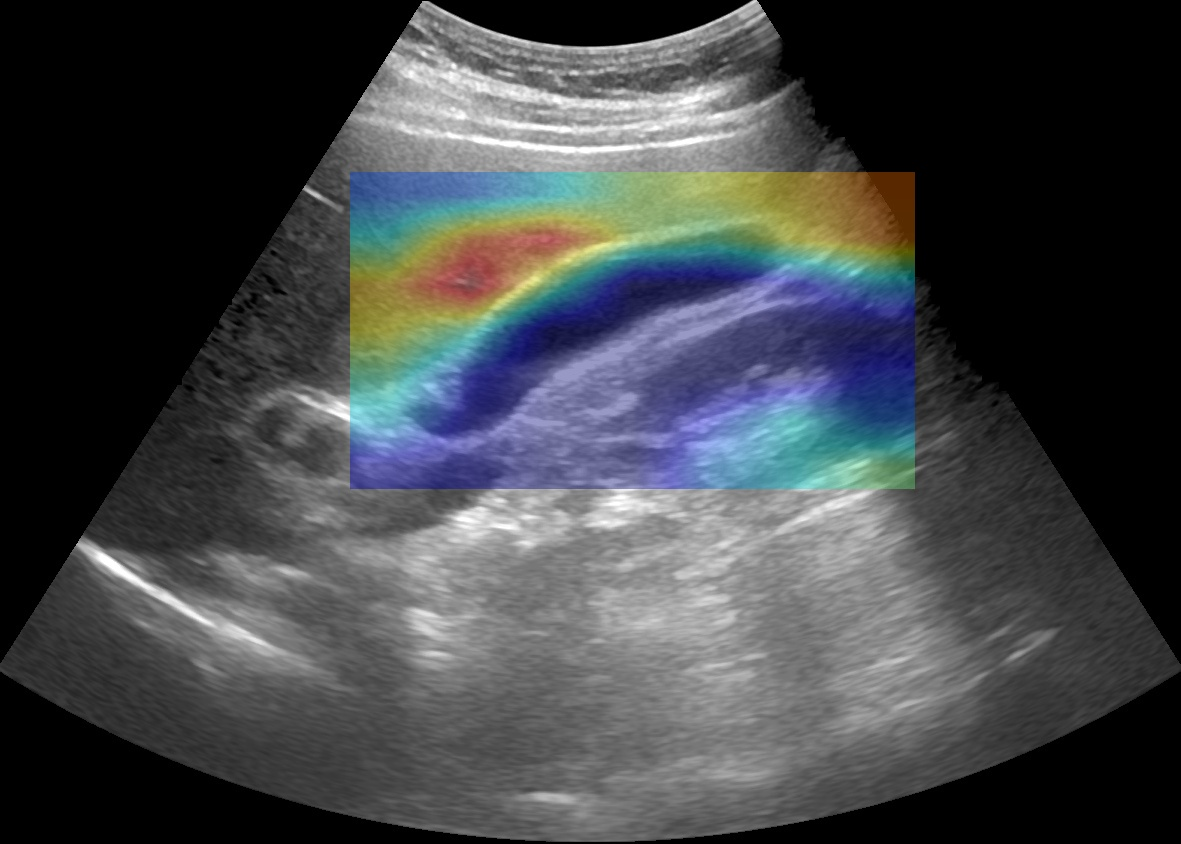
\includegraphics[width=\linewidth,height=8em]{figs/gbcnet/texture-1.jpg}
		\caption{}
		%\label{fig:multi-scale}
	\end{subfigure}
    \begin{subfigure}[b]{0.3\linewidth}
		\centering
		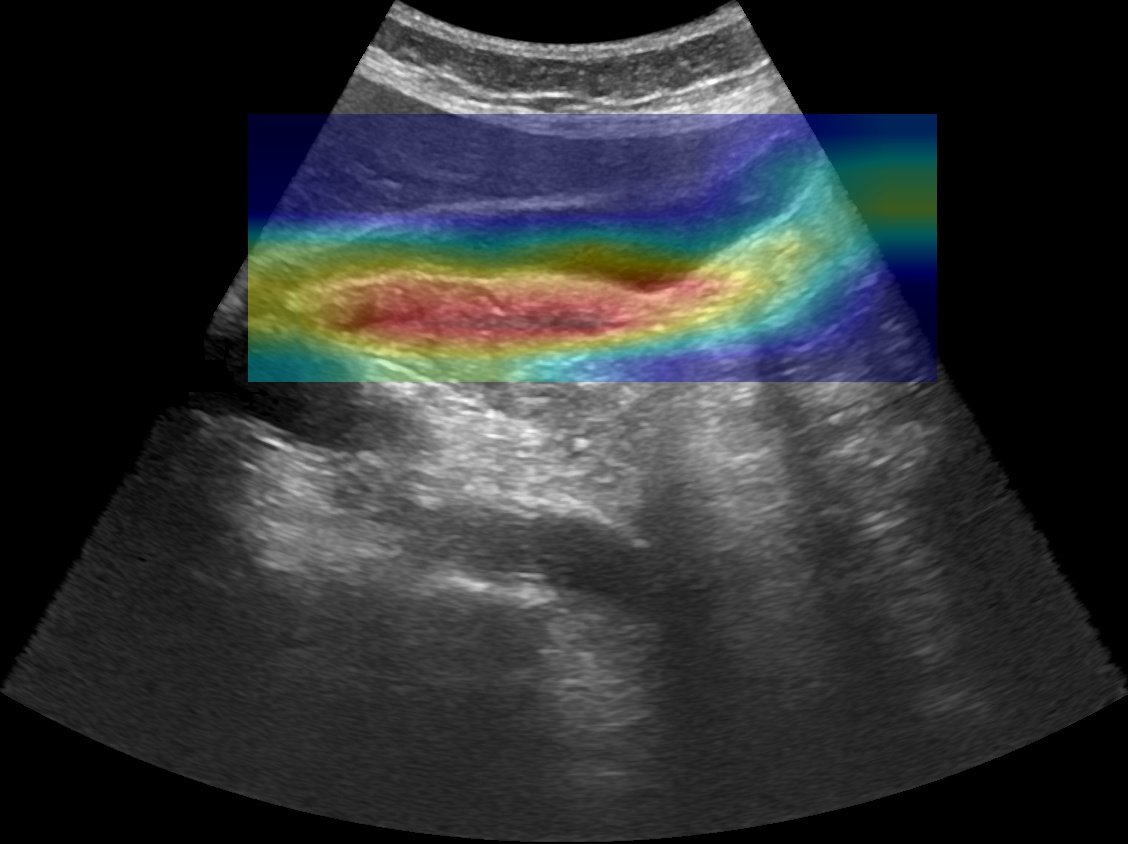
\includegraphics[width=\linewidth,height=8em]{figs/gbcnet/texture-2.jpg}
		\caption{}
		%\label{fig:multi-scale}
	\end{subfigure}
	\begin{subfigure}[b]{0.3\linewidth}
		\centering
		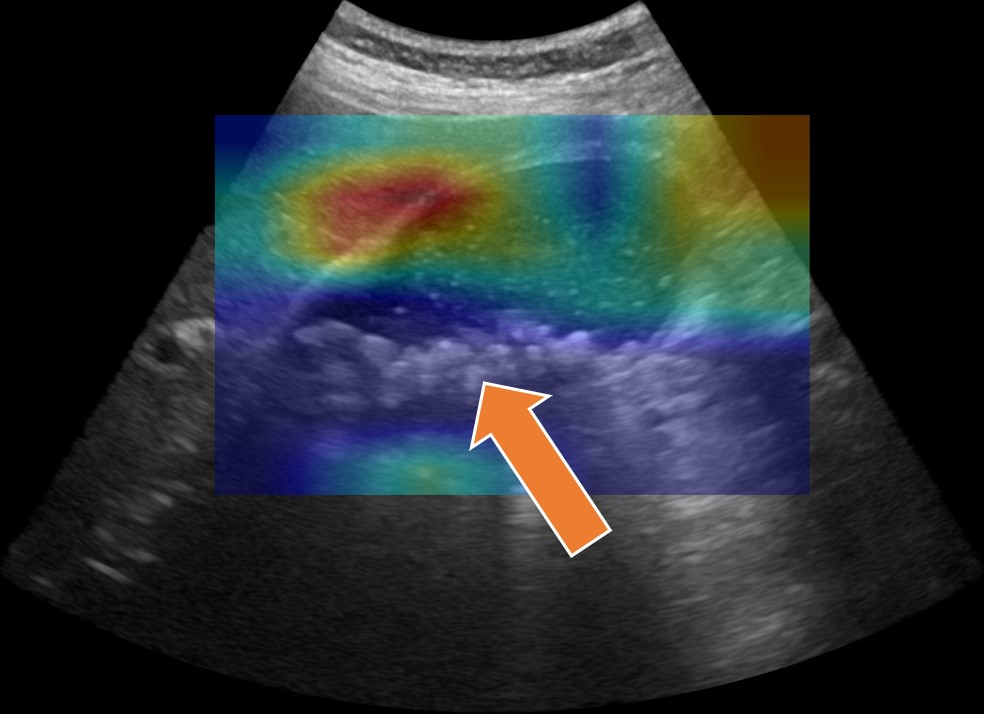
\includegraphics[width=\linewidth,height=8em]{figs/gbcnet/texture-3.jpg}
		\caption{}
		%\label{fig:multi-scale}
	\end{subfigure}
    \caption[Visualization of texture bias]{Grad-CAM visual of GBCNet trained without curriculum showing how the model tends to get biased due to the presence of textures due to noise or organ tissue. GBCNet focuses on - (a) adjacent liver tissues than the normal \gb, (b) the echogenic region below the \gb, and (c) liver textures instead of the stones (highlighted using the arrow).}
    \label{fig:texture_bias_sample}
\end{figure}
%
\begin{figure}[t]
	\centering
	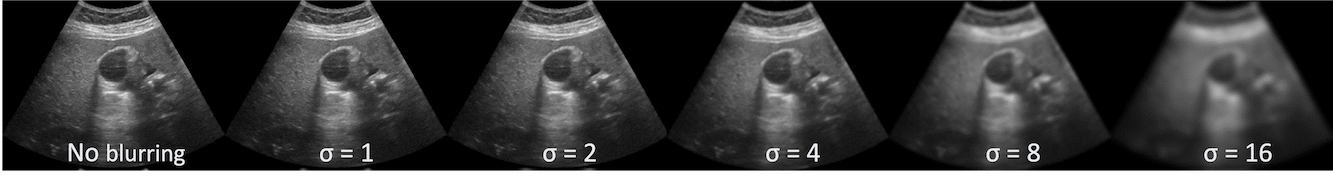
\includegraphics[width=0.95\linewidth]{figs/blur_sample_1.png}
	\caption[Gaussian blurring of USG data samples]{We simulate visual acuity through the Gaussian blur. Increasing $\sigma$ in a Gaussian filter decreases the visual acuity. Notice in the figure that, the effect of textures reduce as the visual acuity decreases and \gb shape and structure become more pronounced.}
	\label{fig:vis_acuity_sample}
\end{figure}

%% Curriculum
\subsection{Visual Acuity Inspired Curriculum}
%
We found that the textures having visual characteristics of soft tissue can adversely affect the performance of GBCNet (\cref{fig:texture_bias_sample}). We propose a curriculum to mitigate the texture bias and improve the classification. We observed that while the MS-SoP classifier is affected by texture bias, the region selection network still maintains a very high recall (\cref{tbl:perf_region}). Hence, we used the curriculum training only on the classifier and not on the region selection network.

\mypara{Visual Acuity in Humans}
%
Visual Acuity (VA) refers to the clarity and sharpness of human vision. Due to the immaturity of the retina and visual cortex, newborn children have very low VA \cite{courage1990visual}. The VA improves with the maturation of the retina and visual cortex. However, for children with congenital cataracts, the cortex matures despite the lenticular opacity. Such children begin their visual activity with higher initial VA. Evidence shows that children with high initial VA suffer to facilitate spatial analysis over expansive areas \cite{vogelsang2018VisualAcuity}.  Low VA renders blurry images that do not contain enough local information for the visual cortex to identify patterns. As a result, the visual cortex tries to increase the receptive field to facilitate spatial analysis over expansive areas and learn global features \cite{kwon2016compensation, smith2009smile}. 

\begin{algorithm}[t]
\small  
	\caption{Proposed Visual Acuity-based Curriculum}
	\label{va_algo}
	\SetAlgoLined
	\KwIn{$D^{\text{train}}$, Dataset of regions cropped from the original USG images.}
	\KwOut{Optimized model parameters $W^*$}
	Initialize $\sigma = \sigma_0$ \;
	%Set warm-up size to be $k'$ \;
	Initialize model parameters to $W$ \;
	
	\For {epoch=$\{1 \ldots, N\}$}{
		\eIf{$\sigma > 0$}{
		    $Z = \phi$ \;
    		\For {$x \in D^{\text{train}}$} {
    			$Z = Z \cup \{x \oast G(\sigma)\}$ \;
    		}
		    train($W, Z$)\;
		}
		{
		    train($W, D^{\text{train}}$) \;
		}
		\If{(epoch $> k'$) and (epoch$\%k == 0$)}{
			$\sigma = \lfloor \sigma/2 \rfloor$ \; 
		}
	}
\end{algorithm}


\mypara{Gaussian Blurring to Simulate Visual Acuity}
%
Gaussian filters are low-pass filters to cloak the high-frequency components of an input. A standard deviation $\sigma$ parameterizes the Gaussian filters. Increasing the $\sigma$ generates a higher amount of blur and low VA when convolved with an image. \cref{fig:vis_acuity_sample} shows how we can decrease the VA by increasing the $\sigma$ of a Gaussian filter. In our experiments, we have varied $\sigma$ from $1$ to $16$ to generate different levels of VA. 

\mypara{Proposed Curriculum}
%
While \cite{vogelsang2018VisualAcuity} demonstrates the improvement in receptive fields by gradually improving the sharpness of images during training, we take this observation further and show that the strategy of training on progressively higher resolution images also reduces the texture bias of a classification model. We propose a visual acuity-based training curriculum (\cref{va_algo}) that starts training the network with blurry and low-resolution \usg images and progressively increase the sharpness of training samples. The initial blurring allows the model to use an extended receptive field and focus on learning the global features such as the shape of the \gb while ignoring any noise or irrelevant textures. In the later phases, the sharp images allow the model to focus on the relevant local features in a controlled manner to make more accurate predictions. 


\section{Dataset Collection and Curation}

\myfirstpara{Data Collection}
%
We acquired data samples from patients referred to PGIMER, Chandigarh (a tertiary care referral hospital in Northern India) for abdominal ultrasound examinations of suspected \gb pathologies. The study was approved by the Ethics Committee of PGIMER. We obtained informed written consent from the patients at the time of recruitment, and protect their privacy by fully anonymizing the data. Minimum 10 grayscale B-mode static images, including both sagittal and axial sections, were recorded by radiologists for each patient using a Logiq S8 machine. We excluded color Doppler, spectral Doppler, annotations, and measurements. Supplementary A %\ref{supp:data_collection} 
contains more details of the data acquisition process.

\mypara{Labeling and ROI Annotation}
%
Each image is labeled as one of the three classes - normal, benign, or malignant. The ground-truth labels were biopsy-proven to assert the correctness. Additionally, in each image, expert radiologists have drawn an axis-aligned bounding box spanning the entire \gb and adjacent liver parenchyma to annotate the \roi. 

\mypara{Dataset Statistics}
%
We have annotated 1255 abdominal \usg images collected from 218 patients from the acquired image corpus. Overall, we have 432 normal, 558 benign, and 265 malignant images. Of the 218 patients, 71, 100, and 47 were from the normal, benign, and malignant classes, respectively. The width of the images was between 801 and 1556 pixels, and the height was between 564 and 947 pixels due to the cropping of patient-related information. 

\mypara{Dataset Splits}
%
The sizes of the training and testing sets are 1133 and 122, respectively. To ensure generalization to unseen patients, all images of any particular patient were either in the train or the test split. The number of normal, benign, and malignant samples in the train and test set is 401, 509, 223, and 31, 49, and 42, respectively. Additionally, we report the 10-fold cross-validation metrics on the entire dataset for key experiments to assess generalization. All images of any particular patient appeared either in the training or the validation split during the cross-validation. 

%results table, pasted here for formatting reasons
\begin{table}[t]
	\centering
	\footnotesize
	%\captionsetup{width=\textwidth}
	%\setlength{\tabcolsep}{10pt}
%	\resizebox{ \linewidth}{!}{%
		\begin{tabular}{lccccccc}
			\toprule[1pt]
			\multirow{2}{*}{\textbf{Method}} & \multicolumn{4}{c}{\textbf{Test Set}} & \multicolumn{3}{c}{\textbf{Cross Val.}} \\
			\cmidrule{2-8}
			& \textbf{Acc.} & \textbf{Acc.-2} & \textbf{Spec.} & \textbf{Sens.} & \textbf{Acc.} & \textbf{Spec.} & \textbf{Sens.}  \\
			\midrule[0.5pt]
			Radiologist A & 70.0 & 81.6 & 87.3 & 70.7 & -- & -- & --  \\
			Radiologist B & 68.3 & 78.4 & 81.1 & 73.2 & -- & -- & --  \\
			\midrule
			VGG16 & 62.3 & 72.1 & 90.0 & 38.1 & 69.3 $\pm$ 3.6 & 96.0 $\pm$ 4.6 & 49.5 $\pm$ 23.4 \\ 
			ResNet50 & 76.2 & 78.7 & 87.5 & 61.9 & 81.1 $\pm$ 3.1 &  92.6 $\pm$ 6.9 & 67.2 $\pm$ 14.7 \\ 
            %0.865 +- 0.070
			InceptionV3 & 77.9 & 85.0 & 87.5 & 80.1 & 84.4 $\pm$ 3.9 & 95.3 $\pm$ 2.9 & 80.7 $\pm$ ~~9.7 \\
			%\midrule
			Faster-RCNN & 71.3 & 77.9 & 76.2 & 81.0 & 75.7 $\pm$ 5.3 & 84.0 $\pm$ 4.6 & 80.8 $\pm$ 10.4 \\
			RetinaNet & 75.4 & 83.6 & 86.3 & 78.6 & 74.9 $\pm$ 7.3 & 86.7 $\pm$ 7.8 & 79.1 $\pm$ ~~8.9 \\
			EfficientDet & 58.2 & 77.9 & 86.3 & 62.0 & 73.9 $\pm$ 8.4 & 88.1 $\pm$ 9.9 & 85.8 $\pm$ ~~6.1 \\
			\midrule%[1.5pt]
			GBCNet & 87.7 & 91.0 & 90.0 & 92.9 & 88.2 $\pm$ 5.1 & 94.2 $\pm$ 3.7 & \textbf{92.3 $\pm$ ~~7.1} \\ 
			GBCNet+VA &\textbf{91.0} & \textbf{95.9} & \textbf{95.0} & \textbf{97.6} & \textbf{92.1 $\pm$ 2.9} & \textbf{96.7 $\pm$ 2.3} & 91.9 $\pm$ ~~6.3 \\
			\bottomrule[1pt]
		\end{tabular}
%	}
	\caption[Comparing GBCNet with baselines for detecting GBC from USG images]{The model performances on the test set and the cross validation (Mean$\pm$SD) in classifying \gbc from USG images. %Apart from the standard accuracy of classifying normal, benign, and malignant \gb, we show the binary classification (malignancy vs. non-malignancy) accuracy on the test set (column Acc.-2). 
    We also report the \gbc detection performance of two expert radiologists on the test set. The radiologists classified each image without accessing the biopsy results or any other patient data. Our model significantly outperforms even the human radiologists. Recall that our ground truth labels are biopsy-proven. The performance of human radiologists in the our study is comparable to that reported in literature \cite{bo2019diagnostic, gupta2020evaluation}. }
	\label{tbl:perf_gbc}
\end{table}

\section{Implementation and Evaluation}
\label{sec:focusmae_impl}
In this section we discuss the specific training setup with FocusMAE for our GBC detection task. We use the FocusMAE-based pretraining on the ViT encoder, enabling it to learn disease representation for the downstream GBC classification task. Following this pretraining phase, the ViT network is fine-tuned for the GBC classification task using classification loss. The pretraining and fine-tuning details including the hyperparameters are discussed here.

\mypara{Pretraining}
%
We implemented our experiments using PyTorch \cite{paszke2019pytorch}. We used Kinetics-400 pretrained weights for MAE weight initialization. Although there is a domain gap in natural and medical image data, studies show that pretraining on natural image data improves network performance on medical imaging tasks \cite{alzubaidi2020transferlearning, cheng2017transfer}.
We used the video sub-sampling scheme discussed in \cref{sec:method_subsample}. We apply random-resize cropping, random horizontal flipping, and random scaling as part of the data augmentations for pretraining. We chose ViT-S as the backbone. 
We use $2 \times 3 \times 16 \times 16$ sized patches on the input video which has size $16\times3\times224\times224$. Consequently, we obtain $\frac{16}{2} \times \frac{3}{3}\times \frac{224}{16} \times \frac{224}{16} = 1568$ tokens for each video.
%We use patch size of $2 \times 3 \times 16 \times 16$, resulting in $\frac{16}{2} \times \frac{3}{3}\times \frac{224}{16} \times \frac{224}{16} = 1568$ tokens for an input video of size $16\times3\times224\times224$.  
The pretraining phase is trained with an AdamW optimizer with LR $0.0001$, layer decay $0.75$, and weight decay $0.05$, for minimizing the MSE loss over 300 epochs. The batch size was 2. Warm-up was done for 3 epochs with LR $0.001$.

\mypara{Fine-tuning}
%
\label{label:impl_ft}
For sub-sampling the videos during fine-tuning, a denser sample rate of 3 was used. We used 16 frames to constitute a clip. From each video, we sampled 5 clips uniformly. During inference, we predict the labels for each of the clips. If any of the clips is predicted as malignant, the entire video is labelled as malignant. We minimized a soft-target cross entropy loss using an AdamW optimizer with LR $10^{-5}$, layer decay $0.75$, and weight decay $0.05$ for 30 epochs. We used a batch size of 4. 

We have used a machine with an Intel Xeon Gold 5218@2.30GHz dual-core processor and 8 Nvidia Tesla V100 32GB GPUs for our experiments. 

\mypara{Evaluation Metrics}
%
We used video-level accuracy, specificity (true negative rate), and sensitivity (true positive rate/ recall) for assessing the video-based GBC identification. %We have used 5-fold cross-validation. 

%
\begin{figure}[t]
	\centering
	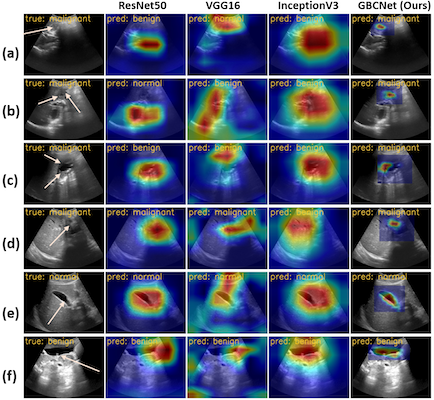
\includegraphics[width=0.62\linewidth]{figs/gbcnet/grad-cam.png}
	\caption[Qaualitative analysis of GBCNet with Grad-CAM visuals]{Grad-CAM visuals and the predictions for ResNet50, VGG16, Inception-V3, and GBCNet. The pathological areas are shown with arrows in the original images. 
	(a) ResNet50 and Inception-V3 focus on the shadow, whereas VGG16 focuses on the echogenic area, and all three fail to detect \gbc. GBCNet accurately focuses on the malignant \gb region invading the liver and detects \gbc.  (b), (c) The baseline networks focus on shadow or noise instead of the cancerous area and mispredict. 
	(d) Although ResNet50 and VGG16 predict malignancy, they fail to precisely focus on the malignant region compared to GBCNet. Inception-V3 failed to classify \gbc. (e), (f) GBCNet pinpoints the discriminating region compared to the baselines for normal and benign \gb regions, respectively. More visuals provided in \cref{fig:supple-2}.} %\ref{supp:cam_vis}.}
	\label{fig:gbc_vis}
\end{figure}

\begin{figure}[t]
	\centering
	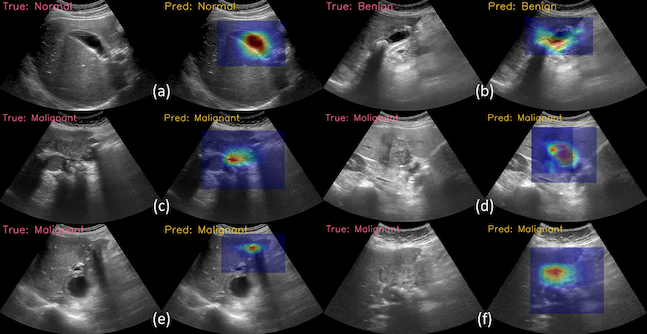
\includegraphics[width=0.7\linewidth]{figs/gbcnet/vis-s-1.png}
	\caption[Additional Grad-CAM visuals for GBCNet]{Sample Grad-CAM visuals of GBCNet with curriculum learning. (a) Normal, (b) Benign, and (c)--(f) Malignant samples.}
	\label{fig:supple-2}
\end{figure}

\section{Experiments and Results}
%
\subsection{Dataset}
%
We have used the image-based GBCU dataset described in \cref{chap:data} for the experiments. We recall that, there is a total of 1255 B-mode static abdominal USG images collected from 218 patients in this dataset. Each image is labeled as one of the three classes - normal, benign, or malignant, based on the biopsy reports. In addition to the classification labels, each image contains an axis-aligned bounding box spanning the entire \gb and adjacent liver parenchyma to annotate the \roi. The \roi in each image is drawn in consensus by two expert radiologists with 10 and 2 years of experience in abdominal radiology. The \roi (bounding box) annotations were used to train the \gb region selection network in the first stage of the GBCNet. The classification network in the second stage was trained using the image class labels. 

\mypara{Dataset Statistics}
%
Overall, we have 990 non-malignant (432 normal and 558 benign) and 265 malignant images. Of the 218 patients, 71, 100, and 47 belong to the normal, benign, and malignant classes, respectively. The width of the images was between 801 to 1556 pixels, and the height was between 564 to 947 pixels due to the cropping of patient-related information. 

\mypara{Dataset Splits}
%
The sizes of the training and testing sets are 1133 and 122, respectively. To ensure generalization to unseen patients, all images of any particular patient were either in the train or the test split. The number of normal, benign, and malignant samples in the train and test set is 401, 509, 223, and 31, 49, and 42, respectively. 
Since the dataset size is small, we also report the 10-fold cross-validation metrics on the entire dataset for key experiments to assess generalization. All images of any particular patient appeared either in the training or the validation split during the cross-validation. 

\subsection{Efficacy of GBCNet over Baselines}
%
We compare GBCNet with three popular deep classifiers, ResNet-50 \cite{resnet}, VGG-16 \cite{vgg}, and Inception-V3 \cite{inception}. We also evaluate the performance of three \sota object detectors, Faster-RCNN \cite{fasterrcnn}, RetinaNet \cite{retinanet}, and EfficientDet \cite{efficientdet} for detecting \gbc. We report the results in \cref{tbl:perf_gbc}. From the reported results, it is clear that baseline networks have poor accuracy for detecting \gbc from \usg images. Grad-CAM \cite{gradcam} visualizations in \cref{fig:gbc_vis} show that the noise, textures, and artifacts significantly influence the decision of baseline classification models. Additionally, \cref{fig:supple-2} shows the sample Grad-CAM visualizations of the predictions using GBCNet (ROI+MS-SoP) with curriculum learning. As highlighted in \cref{sec:usg_artifact_issue}, the standard DNN models tend to focus on the large shadow regions, and as a result, their classification accuracy suffers heavily. The shadow regions resembles the visual characteristics of a normal gallbladder (dark, anoechoic region). Compared to the baselines, GBCNet along-with the proposed MS-SoP classifier precisely focuses on crucial visual cues leading to its superior performance. 
%
\begin{table}[t]
	\centering
	\footnotesize
%	\captionsetup{width=\linewidth}
%    \setlength{\tabcolsep}{6pt}
%	\resizebox{\linewidth}{!}
	\caption[Comparison of the \gb region selection models]{Comparison of the \gb region selection models. We reported 10-fold cross validation (Mean$\pm$SD) of the metrics.}
\label{tbl:perf_region}
\end{table}
%
\begin{figure}[t]
	\centering
	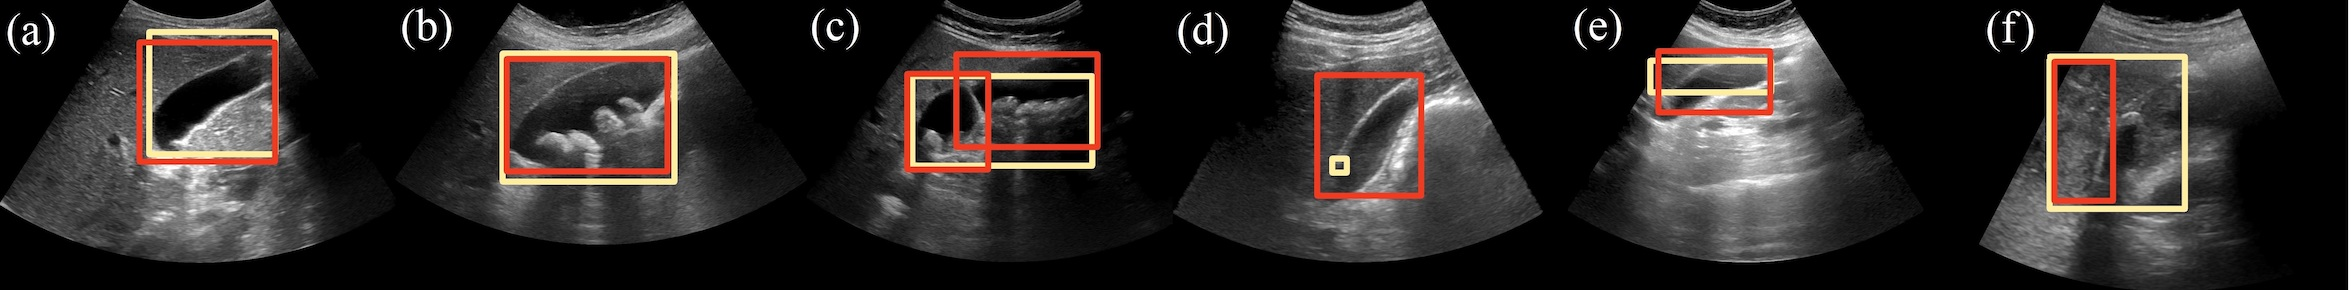
\includegraphics[width = \linewidth]{figs/roi_preds.jpg}%{figs/gbcnet/roi_preds.jpg}
	\caption[Comparison between the ROIs predicted by Faster-RCNN with radiologists]{We visually compare \roi selection by Faster-RCNN (dark red) with the \roi identified by expert Radiologists (light yellow). (a, b) The predicted a\roi matches well with the radiologists' expectations. (c) The model considers the sections partitioned by the \gb wall as separate regions. However, the union of the predicted boxes very closely approximates the actual \gb region. (d, e) Although the radiologist made an error in judging the \roi, Faster-RCNN was able to identify an accurate \roi resulting in a visually superior prediction. (f) The predicted \roi covers only a portion of the area an expert radiologist considered necessary. Even though the region prediction seems inferior compared to the human perception, expert radiologists corroborated that the predicted region captures the \gb invading the liver, a vital visual cue to detect \gbc. \roi samples from other detectors are in Appendix \cref{fig:supple-1}.}
	%\ref{supp:roi_vis}.}
	\label{fig:region_vis}
\end{figure}
%
\begin{figure}[t]
	\centering
	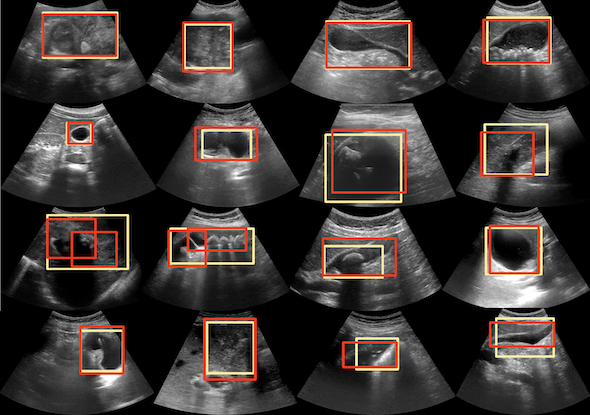
\includegraphics[width=0.7\linewidth]{figs/gbcnet/vis-s-0.png}
	\caption[Additional ROI visuals]{Sample visual results of RoI Detection models. First row - Faster-CNN, second row - YOLOv4, third row - Reppoints, and fourth row - CentripetalNet. Dark red is the ROI prediction by the model and light yellow is expert radiologists' perception of ROI.}
	\label{fig:supple-1}
\end{figure}
%
%\section{Appendix}
%
%
%\subsection{GradCAM Visuals for GBCNet}
%\label{supp:cam_vis}
Figure \ref{fig:supple-2} shows the sample Grad-CAM visualizations of the predictions using GBCNet (ROI+MS-SoP) with curriculum learning. %The blue regions show the most vital regions used by the classifier during prediction. The classifier well emphasized the crucial visual cues during inference.  

% \subsection{Candidate ROI Visuals}
% \label{supp:roi_vis}
% In figure \ref{fig:supple-1}, we show sample predictions of the GB region localization for different models. We also show the region of interest as perceived by the expert radiologists. The localization model is fairly accurate in capturing important regions of the USG image.

%
%
%\mypara{Performance of \gb Region Selection Models}
\subsection{Performance of GB Region Selection Models}
%
\cref{tbl:perf_region} summarizes the performance of various models for localizing the \gb region. For critical tasks such as region selection for cancer detection, recall is more important than precision. Multiple predicted regions can be discarded in the second stage, but missing any potentially malignant region could be disastrous. We note that the Faster-RCNN achieves the highest mIoU out of all the models while maintaining very high recall and excellent precision. Hence, we use Faster-RCNN as the region selection model. In \cref{fig:region_vis} we show the visual comparison of the \gb localization results of Faster-RCNN along with the \rois annotated by the expert radiologists. The model could predict the region of interest accurately in most cases. Although the model's prediction visually differed from the radiologists in some samples, closer inspection revealed that the predicted region retains sufficient visual cues to detect malignancy. In figure \ref{fig:supple-1}, we show additional sample predictions of the GB region localization for different models. 

\begin{table}[t]
	\centering
    \footnotesize
    \begin{tabular}{@{}lccc@{}}
    \toprule[1pt]
    \textbf{Model} & \textbf{Spec.} & \textbf{Sens.} \\
    \midrule[0.5pt]
    ResNet50 &  0.975 $\pm$ 0.024 & 0.829 $\pm$ 0.088\\
    DenseNet121  & 0.968 $\pm$ 0.018 & 0.824 $\pm$ 0.027 \\
    \midrule[0.5pt]
    MS-SoP (ours) & 0.967 $\pm$ 0.027 & 0.871 $\pm$ 0.071 \\
    \bottomrule[1pt]
    \end{tabular}
	\caption[Breast cancer detection results]{The sensitivity and specificity of MS-SoP and two baseline classifiers on breast cancer detection from USG images. We report 5-fold cross-validation on the BUSI dataset.}
\label{tbl:busi}
\end{table}

\begin{table}[t]
	\centering
	\footnotesize
	%\captionsetup{width=\linewidth}
    %\setlength{\tabcolsep}{10pt}
%    \resizebox{ \linewidth}{!}{%
    \begin{tabular}{lcccc}
    \toprule[1pt]
    \multirow{2}{*}{\textbf{Model}} & \multicolumn{2}{c}{\textbf{Orig. Test Set}} & \multicolumn{2}{c}{\textbf{Synth. Test Set}} \\
    & \textbf{Spec.} & \textbf{Sens.} & \textbf{Spec.} & \textbf{Sens.}\\
    \midrule[0.5pt]
    %AR+VGG16 & 51.6 & 56.3 & 88.1 & 55.7 ($\downarrow$) & 62.5 ($\downarrow$) & 88.1 \\
    ROI+VGG16 & 0.838 & 0.572 & 0.787 ($\downarrow$~~6.1\%) & 0.572 \\
    ROI+VGG16+VA & 0.825 & 0.762 & 0.775 ($\downarrow$~~6.1\%) & 0.762 \\
    \midrule
    %AR+ResNet50 & 84.3 & 85.7 & 88.6 & 71.3 ($\downarrow$) & 65.0 ($\downarrow$) & 88.6 \\
    %AR+ResNet50+curriculum & 91.8 & 93.8 & 97.6  & 88.5 ($\downarrow$) & 87.5 ($\downarrow$) & 97.6 \\
    ROI+ResNet50 & 0.863 & 0.857 & 0.650 ($\downarrow$24.7\%)& 0.857 \\
    ROI+ResNet50+VA & 0.938 & 0.857 & 0.887 ($\downarrow$~~5.4\%) & 0.857 \\
    \midrule
    ROI+Inception-V3 & 0.563 & 0.833 & 0.413 ($\downarrow$26.6\%) & 0.833 \\
    ROI+Inception-V3+VA & 0.913 & 0.690 & 0.788 ($\downarrow$13.7\%) & 0.690 \\
    \midrule
    GBCNet & 0.900 & 0.929 & 0.762 ($\downarrow$15.3\%) & 0.929 \\
    GBCNet+VA & 0.950 & 0.976 & 0.850 ($\downarrow$10.5\%) & 0.976 \\
    \bottomrule[1pt]
    \end{tabular}
%    }
    \caption[Robustness of the visual acuity curriculum in tacking texture bias]{Robustness of the curriculum in tacking texture bias while detecting \gbc. We show the performance of using curriculum on four models that apply classifiers on localized \gb region - (a) ROI+VGG16, (b) ROI+ResNet50, (c) ROI+Inception-V3, and (d) GBCNet (ROI+MS-SoP). The relative change (in percentage) in specificity for synthetic test data is shown within parentheses. The sensitivity remains unchanged as the malignant images were not altered. Observe that as compared to the models trained on high-resolution images, our VA-based curriculum is more robust to textures and is able to maintain a lower drop in specificity. The only exception is the ROI+VGG16 model, for which the curriculum training does not lower the drop in specificity. }
    %Also, note how the proposed curriculum is able to improve the performance of all four networks.}
\label{tbl:curr_texture}
\end{table}

\subsection{Applicability of the Proposed Classifier in Breast Cancer Detection from USG Images}
%
We explored the applicability of the proposed MS-SoP classifier on breast cancer detection from \usg images for a publicly available dataset, BUSI \cite{al2020dataset}, containing 133 normal, 487 benign, and 210 malignant images. The images in BUSI are already cropped from original \usg images to highlight only the important regions. Thus, we skip the \roi selection and run the MS-SoP classifier on BUSI. \cref{tbl:busi} shows that the MS-SoP classifier achieves much better sensitivity, which indicates the superiority of the MS-SoP architecture for malignancy identification on \usg images. We note that while breast cancer detection relies on tissue/ mass characterization, \gbc detection is primarily based on wall shape and mass anomaly. %The performance gain using MS-SoP on these two different types of cancers is interesting to note.
\par We remark that, while the MS-SoP classification network was applicable on both tasks, the Visual Acuity-based curriculum may not be suitable for Breast Cancer Detection. Breast cancer detection from USG relies heavily on the textures of the mass/ tissue in the images, as opposed to the wall shape and mass forming anomalies in GBC. Thus, while using a smoothing-based curriculum to bias the learning towards shape features is conducive for GBC detection, it may not aid breast cancer detection.

\begin{figure}[t]
	\centering
	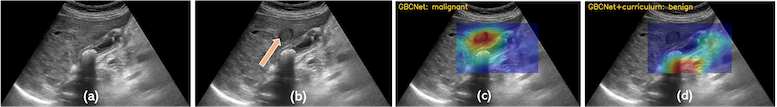
\includegraphics[width=0.9\linewidth]{figs/gbcnet/texture_vis_curr.png}
	\caption[Visualization of the effect of curriculum]{(a) Original image of a benign \gb. The \gb presents a stone and thickened wall. (b) In the synthetic image, we added an artificial tissue-like patch near the benign \gb region (highlighted by the arrow). This patch is not a part of the original \gb, and expert radiologists confirmed that the diagnosis of the \gb is not altered. (c) The textured artificial patch makes the GBCNet biased, and it focuses on the patch to predict the sample as malignant (false-positive). (d) Visual acuity curriculum fixes the texture bias of the GBCNet and helps the network to re-adjust the salient regions to the actual \gb pathology. %and learn the visual cues of a non-malignant \gb such as stone or a thickened wall.
}
	\label{fig:texture_vis}
\end{figure}

\subsection{Efficacy of the Proposed Curriculum}
%
\myfirstpara{Robustness in Tackling Texture Bias}
As described earlier, spurious textures present in \usg images tend to increase the false positives in detecting malignancy. To validate this hypothesis, we created a synthetic test set. We used the method given by \cite{yang2020fda} and added low-level frequencies from malignant images to alter the original texture of normal and benign samples. We also manually added patches looking like soft tissue near the \gb region of normal and benign images. Expert radiologists confirmed that the diagnosis of the \gb pathology is not altered. \cref{tbl:curr_texture} shows that the specificity decreases due to the increase of the false positives. The sensitivity remains unaffected as the prediction for malignant \gb samples was unchanged. The network trained with the proposed curriculum tackles texture bias well and accurately predicts non-malignant samples in synthetic test data. This experiment shows that the proposed curriculum effectively tackles texture bias. \cref{fig:texture_vis} shows a visual sample of how the soft tissue-like texture influences the network's decision and how the curriculum helps the network to rectify the discriminative regions. 

\begin{table}[t]
	\centering
	\footnotesize
%	\captionsetup{width=\linewidth}
%    \setlength{\tabcolsep}{6pt}
%	\resizebox{\linewidth}{!}{%
    \begin{tabular}{@{}lccc@{}}
    \toprule[1pt]
    \textbf{Model} & \textbf{Acc} & \textbf{Spec.} & \textbf{Sens.} \\
    \midrule[0.5pt]
    ROI+VGG16 & 0.533 $\pm$ 0.092 & 0.719 $\pm$ 0.115 & 0.733 $\pm$ 0.179\\
    ROI+VGG16+VA & 0.777 $\pm$ 0.041 & 0.938 $\pm$ 0.030 & 72.0 $\pm$ 0.195\\
    \midrule
    ROI+ResNet50 & 0.766 $\pm$ 0.107 &  0.823 $\pm$ 0.105 & 0.909 $\pm$ 0.111\\
    ROI+ResNet50+VA & 0.854 $\pm$ 0.077 & 0.923 $\pm$ 0.059 & 0.875 $\pm$ 0.091 \\
    \midrule
    ROI+Inception-V3 & 0.718 $\pm$ 0.089 & 0.833 $\pm$ 0.087 & 0.785 $\pm$ 0.214\\
    ROI+Inception-V3+VA & 0.826 $\pm$ 0.046 & 0.931 $\pm$ 0.044 & 0.826 $\pm$ 0.099\\
    \midrule
    % RetinaNet & 74.9 $\pm$ 7.3 &  86.7 $\pm$ 7.8 & 79.1 $\pm$ 8.9\\
    % RetinaNet+VA & 73.3 $\pm$ 6.0 & 92.1 $\pm$ 4.4 & 70.6 $\pm$ 14.2\\
    % \midrule
    GBCNet (ROI+MS-SoP) & 0.882 $\pm$ 0.051 & 0.942 $\pm$ 0.037 & 0.923 $\pm$ 0.071\\
    GBCNet+VA & 0.921 $\pm$ 0.029 &  0.967 $\pm$ 0.023 & 0.919 $\pm$ 0.063\\
    \bottomrule[1pt]
    \end{tabular}
%	}
	\caption[Model performances for training with visual acuity curriculum]{Model performances (10-fold cross-validation) for training with our proposed visual acuity-based curriculum.}
\label{tbl:curr_improve}
\end{table}

\mypara{Performance Improvement with Proposed Curriculum}
We also assess the quantitative performance improvement of models due to the curriculum training in \cref{tbl:curr_improve}. All models show improvement in specificity, which indicates the effectiveness of the proposed blurring-based curriculum in tackling texture bias, and reducing false positives. 

%\subsubsection{Generalization to multiple resolutions}
%%
%To verify how well can the curriculum enhance the generalization capability of \GBCNet at different resolutions, we evaluate the performance of the \GBCNet on the test set at different resolutions. We do this by blurring the test set using different values of $\sigma$ and evaluating GBCNet on these images. Like before, we evaluated the GBCNet without any curriculum and GBCNet with curriculum, anti-curriculum, and the control-curriculum models. The results of this comparison can be seen in \cref{fig:gbc_curr_blur}. The model trained using our proposed curriculum generalizes well across a larger spectrum of image resolutions, and this is an indicator of better spatial understanding than the other models. Note that, the blurred images improve the detection of non-malignant test samples (\cref{fig:spec-test-blur}) for all models. This is an alternate validation of the hypothesis that non-malignant samples (normal and benign) learn better from shape than textures. An interesting observation is that the anti-curriculum performs well at highly blurred (low-resolution) test samples. This can be explained from the fact that anti-curriculum is presented with low-resolution images towards the end of the training cycle. Thus, it maintains the sensitivity better for low-resolution test samples. The curriculum-based GBCNet learns high resolution images towards the later part of the training and thus the sensitivity starts to degrade with low resolution images.

\begin{figure}[t]
	\centering
	\begin{subfigure}[b]{0.23\linewidth}
    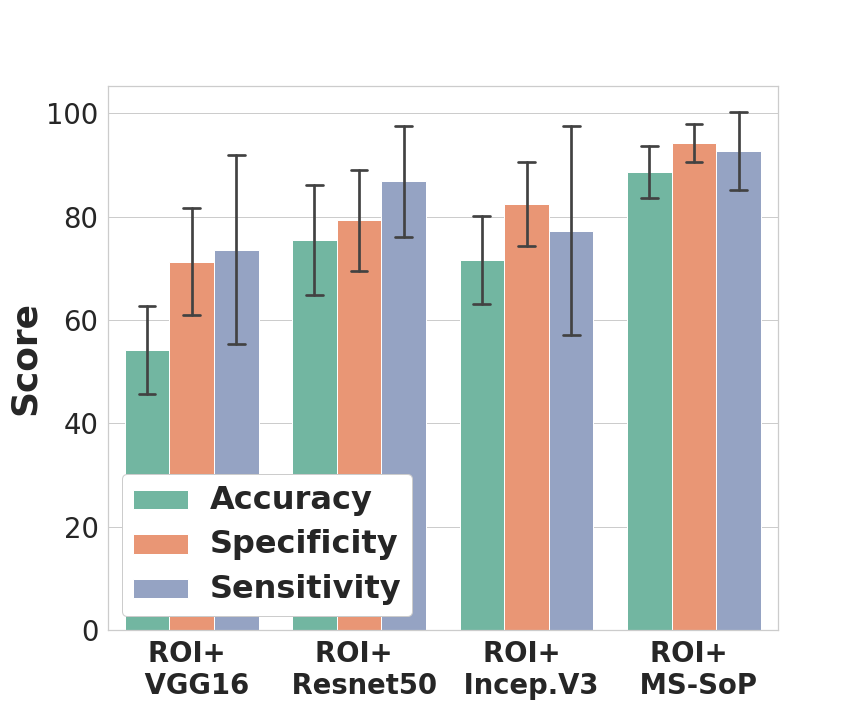
\includegraphics[width=\linewidth]{figs/gbcnet/roi_models.png}
    \caption{}
    \label{fig:perf_attn_models}
    \end{subfigure}
	\begin{subfigure}[b]{0.23\linewidth}
		\centering
		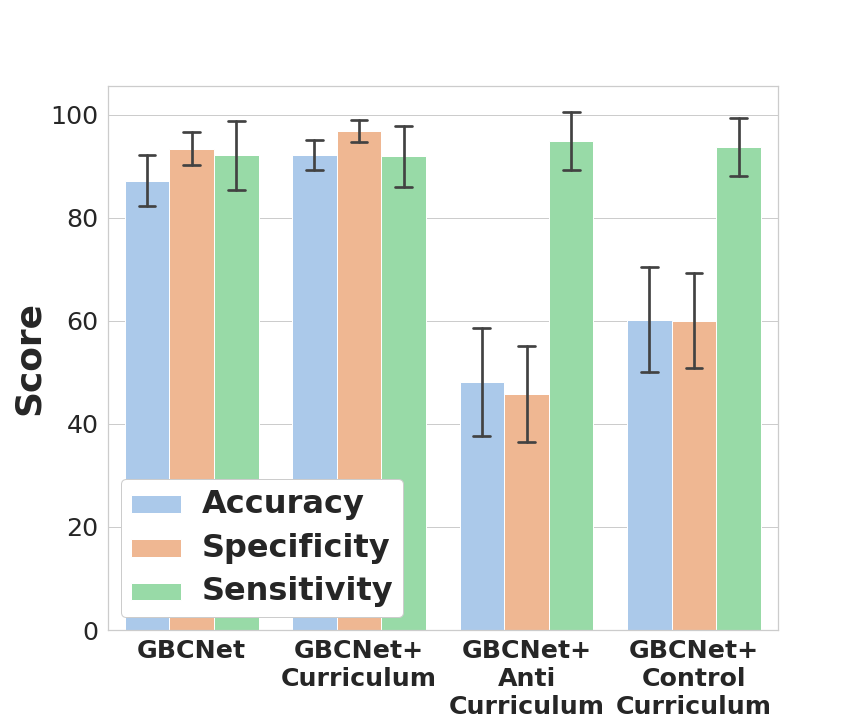
\includegraphics[width=\linewidth]{figs/gbcnet/curr_pred.png}
		\caption{}
		\label{fig:ablation1}
	\end{subfigure}
	%
	\begin{subfigure}[b]{0.23\linewidth}
		\centering
		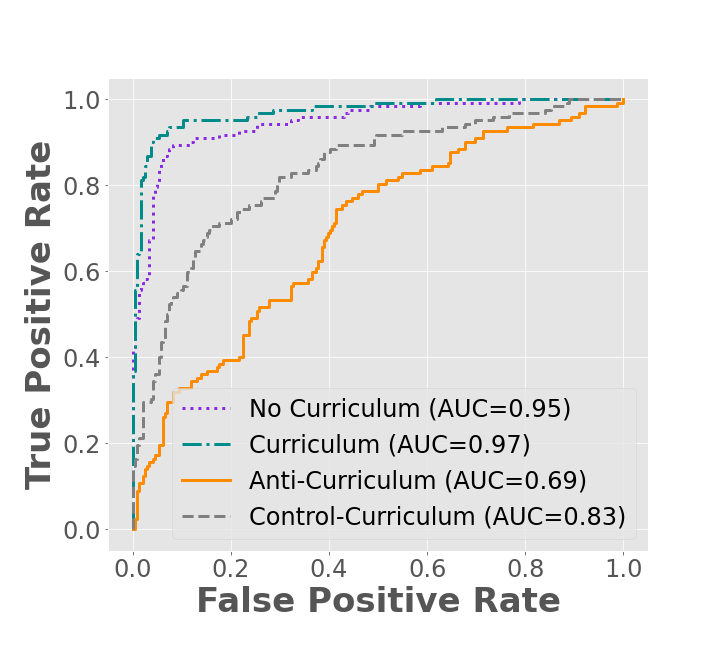
\includegraphics[width=\linewidth]{figs/gbcnet/roc.png}
		\caption{}
		\label{fig:ablation2}
	\end{subfigure}
		\begin{subfigure}[b]{0.23\linewidth}
		\centering
		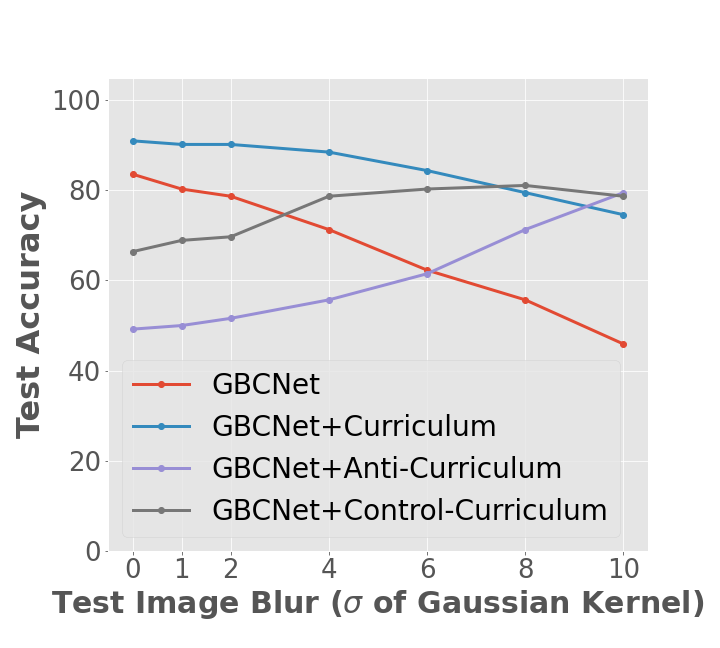
\includegraphics[width=\linewidth]{figs/gbcnet/acc-mr.png}
		\caption{}
		\label{fig:ablation3}
	\end{subfigure}
	\caption[Ablation study]{Ablation study. (a) Comparison of accuracy, specificity, and sensitivity for applying different classification networks (VGG16, ResNet50, Inception-V3, and MS-SoP) on the localized \gb. We have reported the 10-fold cross validation results. (b) The efficacy of the proposed training regime in terms of accuracy, specificity, sensitivity. (c) ROC-AUC for different training regimes on the test set. (d) The proposed curriculum generalizes better at different resolutions. }
	\label{fig:diff_images}
\end{figure}

\subsection{Ablation Study}
%
\myfirstpara{Choice of Classifier in GBCNet}
%
We have plugged in other deep classification networks in place of the proposed MS-SoP classifier in the GBCNet framework. \cref{fig:perf_attn_models} summarizes the results. The MS-SoP classifier on GBCNet provides the best \gbc detection accuracy. Using the classifiers on the \rois improves the sensitivity and accuracy for ResNet50 and VGG16. However, the drop in specificity results in performance degradation for Inception-V3 as the sensitivity was not improved.  

\mypara{Choice of Training Regime}
%
We used the proposed GBCNet model to assess the influence of the visual acuity-based curriculum. We compare the curriculum with two possible alternatives - (i) \emph{anti-curriculum} that initially trains with high resolution and progressively lowers the resolution, and (ii) \emph{control-curriculum} where the samples are not sorted resolution-wise, and the curriculum contains a random set of blurred samples. Note that the control-curriculum can also be thought of using Gaussian blurring as a data augmentation where the probability of choosing a particular $\sigma$ is equal to the fraction of epochs the $\sigma$ used during the curriculum. \cref{fig:ablation1} and \ref{fig:ablation2} show the performance of the various curriculum strategies on the performance on GBCNet.  %\cref{fig:gbc_curr_blur} shows the ROC with the AUC for GBCNet with different curriculum. 
%Additionally, \cref{tbl:curr_texture} shows the performance improvement of attention region-based classifiers when trained with the proposed curriculum.
Further, to understand how various curriculum strategies affect a model's generalization at different resolutions, we blur the test set using different values of $\sigma$ and evaluate the models on these images (\cref{fig:ablation3}). 
%The results of this comparison can be seen in \cref{fig:ablation3}. 
We see that the model trained using the proposed curriculum generalizes well across different image resolutions, which is an indicator of better spatial understanding.

\begin{table}[t]
	\centering
	\footnotesize
%	\captionsetup{width=\linewidth}
%    \setlength{\tabcolsep}{6pt}
%	\resizebox{\linewidth}{!}{%
    \begin{tabular}{@{}lccc@{}}
    \toprule[1pt]
    \textbf{Model} & \textbf{Spec.} & \textbf{Sens.} \\
    \midrule[0.5pt]
    ROI+MS-SoP (GBCNet) & 0.942 $\pm$ 0.037 & 0.923 $\pm$ 0.071 \\
    ROI+MS-SoP (channel-wise pooling) & 0.904 $\pm$ 0.047 & 0.861 $\pm$ 0.068  \\
    ROI+MS-SoP (spatial pooling) & 0.900 $\pm$ 0.064 & 0.882 $\pm$ 0.064 \\
    ROI+MS (w/o SoP) & 0.887 $\pm$ 0.060 & 0.872 $\pm$ 0.064 \\
    ROI+SoP (w/o MS) & 0.914 $\pm$ 0.048 & 0.854 $\pm$ 0.079 \\
    \bottomrule[1pt]
    \end{tabular}
%	}
	\caption[Ablation of the proposed MS-SoP network]{Ablation of Ms-SoP. We show the specificity and sensitivity of MS-SoP with two alternatives - MS-SoP with (i) only channel-wise and (ii) only spatial pooling. We also show the efficacy of using multi-scale and second-order pooling in conjunction.}
\label{tbl:ms-sop-ablation}
\end{table}

\mypara{Components of the MS-SoP Classifier}
%
We present the ablation study on the MS-SoP classifier in \cref{tbl:ms-sop-ablation}. We show the effect of the multi-scale and second-order pooling components on the specificity and sensitivity of the model. We also show the relevance of the channel-wise and spatial pooling in the second-order pooling.
\chapter{Conclusion and Future Directions}
%
\label{chap:conclusion}
%
Finally, we come to the conclusion of the thesis. We present a concise overview of the contributions, followed by the limitations, future directions, and prospects of our work.

\par In this thesis, we have addressed the critical yet hitherto overlooked problem of Gallbladder Cancer (GBC) detection from Ultrasound Sonography (USG). We commence our exploration in \Cref{chap:intro} by discussing the background and motivation behind tackling the problem of automated detection of GBC. 
Following that, we set the stage by emphasizing USG as a diagnostic imaging modality, and its relevance in GBC diagnosis. We also highlighted the basics of USG and the unique challenges associated with USG in the context of GBC detection in \Cref{chap:usg}. \Cref{chap:data} delved into the data acquisition protocol and provided a comprehensive dataset description for the study.

\par In \Cref{chap:gbcnet}, we addressed the challenges related to \usg images, including sensor noise, acoustic shadows, echogenic textures, small pathology size, and variations in appearance of malignancy. To tackle these issues, we introduced \gbcnet \cite{basu2022surpassing}, a novel architecture specifically designed to address the complexities of \usg imaging. Employing a deep detection approach, \gbcnet initially identifies regions of interest to nullify the impact of noise. Subsequently, a novel specialized classification network (MS-SOP) is applied to learn rich representations of malignancy. Additionally, we introduced a smoothing-based curriculum inspired by the human visual acuity to train the classifier, aiming to alleviate texture bias originating from adjacent organs and tissues.

%we attack the problems associated with USG images due to the sensor noise and artifacts such as shadows and textures, and the viewpoint variations arising from the handheld sensor. We develop GBCNet \cite{basu2022surpassing}, a new architecture to solve the problems associated with USG imaging. We have used a deep detection approach to first identify the regions of interest to focus on from the image in order to nullify the effect of the noise. Following this, a novel specialized classification network (MS-SOP) is used for learning the rich representation of the cancers. In addition, we introduce a new Gaussian smoothing-based curriculum to train the classifier in order to mitigate the texture bias arising from the adjacent organs and tissues.

\par While \gbcnet exhibits significantly superior performance compared to expert radiologists and state-of-the-art CNN models, its dependence on bounding box annotations for training the detection component proves to be a bottleneck. The specialized nature of these annotations requires expert medical professionals. In response, \Cref{chap:limited} and \Cref{chap:wsod} address a crucial challenge in medical image computing -- efficient learning with limited supervised data. We explore two distinct avenues to overcome this challenge. Firstly, in \Cref{chap:limited}, we leverage unlabeled USG video data to acquire rich representations for the downstream GBC classification task on USG images \cite{basu2022unsupervised}. We introduce an unsupervised contrastive framework that exploits both intra-video and cross-video negatives, going beyond the conventional approach of mining only cross-video negatives as suggested in previous literature. Secondly, in \Cref{chap:wsod}, we formulate GBC detection as weakly supervised object detection using only image-level labels \cite{basu2023gall}. We enhance the DETR architecture with a multiple-instance learning framework, effectively addressing weakly supervised GBC detection and achieving competitive performance without the need for costly bounding box labels or additional video data.
%Although \gbcnet provides far superior performance as compared to the expert radiologists and the state-of-the-art CNN models, the reliance on the bounding box annotations to train the detection part of \gbcnet proves to be a bottleneck. The specialized nature of the annotations necessitates extensively trained medical professionals to annotate data. In response, we tackle in \Cref{chap:limited} a key challenge in the field of medical image computing -- learning efficiently with limited supervised data. We have explored two distinct avenues to solve the challenge. We exploited the unlabelled USG video data to learn rich representations for the downstream GBC classification task on USG images. We introduced an unsupervised contrastive framework to exploit both intra-video and cross-video negatives as opposed to mining only cross-video negatives as suggested in previous literature. In another approach, we formulated the GBC detection as a weakly supervised object detection using only image-level labels. We augmented the DETR architecture with the multiple instance learning framework towards solving the weakly supervised GBC detection, and achieved competitive performance even without costly bounding box labels or additional video data. 

\par In \Cref{chap:radformer}, we delve into another fundamental challenge -- interpretability. Interpretable decision-making in automated disease detection is crucial from a clinical standpoint. To meet this need, we introduce a novel deep neural network architecture, RadFormer, designed to learn interpretable representations for the detection of  GBC from USG images \cite{basu2023radformer}. RadFormer utilizes a local bag-of-word style feature embedding approach to generate explanations that are not only human-readable but also aligned with radiological reporting standards.

\par Finally, in \Cref{chap:focusmae}, we advocate a paradigm shift to USG video-based detection from the previously employed image-based detection approaches. The need to select the key individual frames in image-based detection is susceptible to operator bias, and single images may lack conclusive features of malignancy. Embracing video-based models offers clinical streamlining as they eliminate the need to select the pivotal frames and leverage rich spatiotemporal information for more accurate GBC detection.

\section{Limitations and Scope of the Work}
%
\subsection{Limitations}
\mypara{No Testing on Real-Time Patients}
%
A limitation of our study pertains to the absence of real-time patient testing, a critical aspect in ensuring the translational impact of our methodologies. The data used in the current study is retrospective in nature, and the practical applicability and robustness of our proposed solutions remain uncertain in real-time patients. Real-time patient testing introduces a dynamic environment with inherent complexities and variations that might not be fully captured in controlled experimental conditions. This limitation calls for future research efforts to bridge the gap between simulated models and actual clinical scenarios. %, promoting the development of more practical and reliable solutions for real-world healthcare applications.

\mypara{Single Center Study}
%
Our research relies on data obtained from a single medical center, and this exclusive focus introduces a limitation regarding the external validity and generalizability of our findings. It is noteworthy that our data collection center is a top tertiary care referral hospital in Northern India, attending both local and far-off patients from different states and localities. Due to this rich demographic variation, our single-center data contains a high degree of patient variation manifesting different sub-types of the disease. However, we acknowledge the limitations of single-center data in terms of limited variation in acquisition equipment and the number of radiologists involved. The dynamics within a single center may not fully encapsulate the broader variations present in diverse healthcare settings. 

\mypara{Not Identified Early Stage GBC}
%
Our work did not tackle the problem of identifying the early stage of the Gallbladder malignancy. Identifying the signs of early stage GBC to provide treatment alternatives is a desirable outcome for clinical setup. However, the aggressive nature of GBC makes the study difficult. 

\subsection{Scope of the Work and Generalizability}
In this work, we have addressed some of the key challenges such as the presence of acoustic shadows, bias to echogenic textures, small objects (pathology), variable appearance owing to non-regular anatomy, and limited data in detecting GBC from Ultrasound with DNN models. The techniques and methods developed in this thesis, such as focused regions-of-interest, smoothing-based curriculum, multi-scale features, second-order feature attention, and global-local features, address some of the key challenges inherent to ultrasound-based GBC detection. The lack of annotated data is tackled through self-supervised pretraining and weakly supervised detectors. The video-based classification method in \Cref{chap:focusmae} helps mitigate issues of operator bias.  Our techniques were demonstrated to solve the problem of GBC detection from ultrasound in the single center retrospective data settings. Nonetheless, the methods developed in this thesis address some of the core challenges of ultrasound-based GBC detection, such as presence of acoustic shadow, echogenic textures, variability in appearance owing to non-regular anatomy. We do not expect our methods to show catastrophic failure in case of unseen data. In fact, we have recently accessed image data of 9 patients (6 benign, 3 malignant) from another tertiary care hospital in Northern India, and were able to run the inference on this data using the RadFormer model (state-of-the-art image-based technique) trained on our original dataset. RadFormer showed 100\% sensitivity (all 3 malignant cases detected correctly) and 83.3\% specificity (5 out of 6 benign cases detected correctly). Although this is a minimal dataset, the results are indicative of the generalization capability of the techniques to unseen data. However, due to the acquisition shift owing to variation in ultrasound machines and operator variability, the outcomes derived from the current study may change with the diverse conditions encountered in multi-center healthcare environments, and result in performance drop. Consequently, caution should be exercised when extrapolating the results to a more extensive, varied population, emphasizing the need for future research encompassing multiple centers.% to enhance the reliability and generalizability of our conclusions.


\section{Future Directions}

\subsection{Translation to Clinical Settings}
%
In our commitment to advancing the translation of research into practical applications, we are actively engaged in exploring the real-world potential of the methodologies developed in this thesis. One avenue of implementation involves deploying the developed models and algorithms onto an Internet-of-Things (IoT) device. This initiative aims to assess the feasibility and performance of the models in a real-time, dynamic healthcare environment. We have shared the IoT device with PGIMER Chandigarh for testing on real-time patients and providing valuable insights into the adaptability and effectiveness of our proposed solutions in a clinical setting. Furthermore, to enhance accessibility and community-level impact, we have established a proof-of-concept web application. The application will be hosted on IIT Delhi's cloud infrastructure, providing a platform for radiologists within the community to leverage the developed models as a secondary resource for improved GBC detection. We seek to democratize access to advanced diagnostic tools, potentially transforming the landscape of GBC detection by empowering community-level radiologists with cutting-edge technology. %Through these practical implementations, we aim to bridge the gap between academic research and real-world healthcare applications, contributing to the development of more practical and reliable solutions.


\subsection{Domain Adaptation/ Generalization – Multi-Center Study}
%
It is imperative to address the domain shift in medical data arising from variations in patient demographics, scanning devices, and radiologist expertise across different hospitals. At present, our study is limited to a specific center, and addressing the challenge of domain adaptation or generalization is crucial for the broader applicability of our models. A future direction will be to focus on mitigating the impact of varying data distributions across hospitals, ensuring the robustness and effectiveness of our models in diverse healthcare settings. 
%To tackle the domain adaptation/generalization problem, we are actively working on the development of models capable of adapting to the nuances of hospitals across different geographic locations. This involves designing algorithms that can seamlessly generalize across diverse datasets, accounting for the inherent variations present in medical data from distinct sources.
In line with these aspirations, we have initiated efforts to acquire data from various hospitals across the country. The nationwide data collection initiative is aimed at creating a more diverse and representative dataset that encapsulates the heterogeneity present in medical data across different healthcare institutions. By incorporating data from multiple sources, we aim to enhance the generalizability and real-world effectiveness of our models, paving the way for more robust and widely applicable solutions in the domain of medical image analysis.

\subsection{Applicability of Foundation Models}
%
%Foundation models have recently gained huge popularity in a plethora of applications. However, its applicability in medical vision is not straight forward due to the paucity of data, and the safety critical nature of the tasks. Though there are some attempts in literature \cite{xraygpt, medsam}, the systematic study of adopting large/ foundation models for medical computer vision is largely unexplored.
Foundation models have recently witnessed immense popularity and widespread adoption across various applications, demonstrating their effectiveness in diverse domains. However, their application in medical computer vision is a complex endeavor, primarily attributed to the scarcity of data and the safety-critical nature of tasks within the healthcare domain. While some preliminary attempts have been made in the literature, such as in the cases of X-ray analysis \cite{xraygpt} and medical image segmentation \cite{medsam}, the systematic exploration and study of adopting large or foundation models for medical computer vision remain largely unexplored.

\subsection{Self-supervised Learning for USG}
%
Addressing the challenge of learning from limited supervised data, especially in the context of ultrasound (USG) imaging, remains a significant hurdle in medical image computing. In this work, we have investigated a contrastive framework utilizing temporal distance as a surrogate for a similarity measure. However, given the operator's reliance on USG, anomalies may reappear in distant frames if a radiologist re-evaluates an organ later during the same scan, leading to potential similarity conflicts. Existing works on self-supervised learning for USG primarily employ techniques like reshuffling of frames \cite{reshuff}, which, given the 2D nature of USG scans of 3D organs, might not be optimal. Exploring appropriate techniques for robust self-supervised learning from USG data presents an important avenue for future research.

\subsection{Multimodal Learning}
%
%In this work, we have explored solely the radiology images (USG) without incorporating additional clinical or radiomic information. Future research opportunities lie in harnessing diverse channels of information, potentially significantly boosting diagnostic performance.
We have exclusively explored radiology images, specifically USG, without integrating additional clinical or radiomic information. Future research endeavors present exciting opportunities to harness diverse channels of information, potentially leading to a substantial enhancement in diagnostic performance.
%The current focus on radiology images serves as a foundational step, and the inclusion of complementary data sources such as clinical information and radiomic features holds promise for a more comprehensive understanding of medical conditions. 
Integrating these additional channels of information can provide a holistic view, enabling the development of more robust and accurate diagnostic models. By leveraging the synergies among various data modalities, future research can unlock new dimensions in medical image analysis, ultimately advancing the capabilities of diagnostic tools and contributing to improved patient care.

\subsection{Discovering Hidden Features with AI}
%
%Our observations indicate that RadFormer generates neural features highly correlated with malignancy, but they do not align with the RADS features used by radiologists. Exploring and understanding the clinical nature of AI-based features and leveraging their synergy with human-used features present promising avenues for future research.
Our observations suggest that RadFormer produces neural features that exhibit a high correlation with malignancy. However, these features do not align with the Radiology Data Systems (RADS) features commonly utilized by radiologists. There is a disjunction between AI-generated features and those traditionally employed by human radiologists.

Exploring and comprehending the clinical nature of AI-generated features and, more importantly, investigating the synergies that can be harnessed between these AI-based features and those utilized by human experts present promising avenues for future research. Bridging the gap between AI-derived features and human-interpretable features can potentially lead to more clinically relevant models, fostering a collaborative and complementary relationship between AI and human expertise in medical image analysis.

\par %In conclusion, we have undertaken a comprehensive exploration of detecting GBC from USG images and videos, and made contributions to the core challenges posed by the problem. We have also identified the future directions and extension of this work with translational impact. The contributions in this thesis cover novel architectures, training methods, and new public datasets with the hope of helping to improve patient care and the bleak survival statistics for GBC. 
\section{Closing Remarks}
%
In summary, our endeavor encompassed a thorough investigation into the detection of GBC from USG images and videos, resulting in significant contributions to the fundamental challenges posed by the problem. The contributions presented in this thesis span novel architectures, innovative training methods, and the creation of new public datasets.
The identified future directions and potential extensions of this work aim to translate the contributions made by this thesis into meaningful improvements in patient care and the overall survival statistics for individuals affected by GBC. The overarching goal is to enhance the effectiveness of automated GBC detection, thereby making a positive impact on clinical practices and patient outcomes.


%%%%%%%%% REFERENCES
\clearpage
{\small
\bibliographystyle{ieee_fullname}
\bibliography{gbc-ref}
}

%%%%%%%%% SUPPLEMENTARY
% \clearpage
% \appendix
% \beginsupplement
% \section*{Supplementary Material}

\maketitle

\appendix
\beginsupplement


\end{document}
